\documentclass[11pt]{aghdpl}
% \documentclass[en,11pt]{aghdpl}  % praca w języku angielskim

% Lista wszystkich języków stanowiących języki pozycji bibliograficznych użytych w pracy.
% (Zgodnie z zasadami tworzenia bibliografii każda pozycja powinna zostać utworzona zgodnie z zasadami języka, w którym dana publikacja została napisana.)
\usepackage[english,polish]{babel}

% Użyj polskiego łamania wyrazów (zamiast domyślnego angielskiego).
\usepackage{polski}

\usepackage[utf8]{inputenc}

% dodatkowe pakiety

\usepackage{mathtools}
\usepackage{amsfonts}
\usepackage{amsmath}
\usepackage{amsthm}

% --- < bibliografia > ---

\usepackage[
style=numeric,
sorting=none,
%
% Zastosuj styl wpisu bibliograficznego właściwy językowi publikacji.
language=autobib,
autolang=other,
% Zapisuj datę dostępu do strony WWW w formacie RRRR-MM-DD.
urldate=iso8601,
% Nie dodawaj numerów stron, na których występuje cytowanie.
backref=false,
% Podawaj ISBN.
isbn=true,
% Nie podawaj URL-i, o ile nie jest to konieczne.
url=false,
%
% Ustawienia związane z polskimi normami dla bibliografii.
maxbibnames=3,
% Jeżeli używamy BibTeXa:
backend=bibtex
]{biblatex}

\usepackage{csquotes}
% Ponieważ `csquotes` nie posiada polskiego stylu, można skorzystać z mocno zbliżonego stylu chorwackiego.
\DeclareQuoteAlias{croatian}{polish}

\addbibresource{bibliografia.bib}

% Nie wyświetlaj wybranych pól.
%\AtEveryBibitem{\clearfield{note}}


% ------------------------
% --- < listingi > ---

% Użyj czcionki kroju Courier.
\usepackage{courier}

\usepackage{listings}
\lstloadlanguages{TeX}

\lstset{
        literate={ą}{{\k{a}}}1
           {ć}{{\'c}}1
           {ę}{{\k{e}}}1
           {ó}{{\'o}}1
           {ń}{{\'n}}1
           {ł}{{\l{}}}1
           {ś}{{\'s}}1
           {ź}{{\'z}}1
           {ż}{{\.z}}1
           {Ą}{{\k{A}}}1
           {Ć}{{\'C}}1
           {Ę}{{\k{E}}}1
           {Ó}{{\'O}}1
           {Ń}{{\'N}}1
           {Ł}{{\L{}}}1
           {Ś}{{\'S}}1
           {Ź}{{\'Z}}1
           {Ż}{{\.Z}}1,
        basicstyle=\footnotesize\ttfamily,
}

% ------------------------

\AtBeginDocument{
        \renewcommand{\tablename}{Tabela}
        \renewcommand{\figurename}{Rys.}
}

% ------------------------
% --- < tabele > ---

\usepackage{array}
\usepackage{tabularx}
\usepackage{multirow}
\usepackage{booktabs}
\usepackage{makecell}
\usepackage{tikz}
\usepackage{pifont}
\usepackage{subcaption}
\usepackage{graphicx}
\usepackage{float}
\usepackage[flushleft]{threeparttable}

% defines the X column to use m (\parbox[c]) instead of p (`parbox[t]`)
\newcolumntype{C}[1]{>{\hsize=#1\hsize\centering\arraybackslash}X}
\newcommand{\xmark}{\ding{55}}%
\newcommand{\cmark}{\ding{51}}%
%---------------------------------------------------------------------------

\author{Radosław Sajdak}
\shortauthor{R. Sajdak}

%\titlePL{Przygotowanie bardzo długiej i pasjonującej pracy dyplomowej w~systemie~\LaTeX}
%\titleEN{Preparation of a very long and fascinating bachelor or master thesis in \LaTeX}

\titlePL{Opracowanie urządzenia wykrywającego wypadek rowerowy z powiadamianiem GSM}
\titleEN{Development of a bicycle accident detection device with GSM notification}


\shorttitlePL{Opracowanie urządzenia wykrywającego wypadek rowerowy} % skrócona wersja tytułu jeśli jest bardzo długi
\shorttitleEN{Development of a bicycle accident detection device}

\thesistype{Praca dyplomowa inżynierska}
%\thesistype{Master of Science Thesis}

\supervisor{dr inż. Łukasz Krzak}
%\supervisor{Marcin Szpyrka PhD, DSc}

\degreeprogramme{Elektronika i Telekomunikacja}
%\degreeprogramme{Computer Science}

\date{2022}

\department{Katedra Elektroniki}
%\department{Department of Applied Computer Science}

\faculty{Wydział Informatyki, Elektroniki,\protect\\[-1mm] i Telekomunikacji}
%\faculty{Faculty of Electrical Engineering, Automatics, Computer Science and Biomedical Engineering}

\acknowledgements{Serdecznie dziękuję \dots tu ciąg dalszych podziękowań np. dla promotora, żony, sąsiada itp.}


\setlength{\cftsecnumwidth}{10mm}

%---------------------------------------------------------------------------
\setcounter{secnumdepth}{4}
\brokenpenalty=10000\relax

\begin{document}

\titlepages

% Ponowne zdefiniowanie stylu `plain`, aby usunąć numer strony z pierwszej strony spisu treści i poszczególnych rozdziałów.
\fancypagestyle{plain}
{
        % Usuń nagłówek i stopkę
        \fancyhf{}
        % Usuń linie.
        \renewcommand{\headrulewidth}{0pt}
        \renewcommand{\footrulewidth}{0pt}
}

\setcounter{tocdepth}{2}
\tableofcontents
\clearpage

\chapter{Wstęp}
\label{cha:wstep}

Obecny rozwój mikroprocesorów, pozwala na tworzenie coraz bardziej złożonych urządzeń. Rozwój układów o niskim zużyciu energii, popycha elektronikę w kierunku małych, wielofunkcyjnych urządzeń. Połączenie tych dwóch procesów pozwala na stworzenie elastycznych urządzeń, których zastosowanie może zmieniać się jedynie dzięki oprogramowaniu.

%---------------------------------------------------------------------------

\section{Cele pracy}
\label{sec:celePracy}

Rowerzyści górscy, podczas samotnych wypraw rowerowych, wielokrotnie zastanawiają się, co w sytuacji, gdy ulegną wypadkowi podczas samotnej wyprawy?
Jak długo nikt nie wezwie pomocy? W ten sposób, powstał pomysł stworzenia urządzenia asystującego.
\newline
Celem pracy było stworzenie innowacyjnego urządzenia wykrywającego upadek na rowerze. Urządzenie miało być przymocowane do ramy roweru. Urządzenie, informację o wypadku wysyła przy użyciu modemu LTE-M opartego o interfejs szeregowy UART. Za lokalizowanie urządzenia, odpowiadać będzie moduł GPS oparty o magistralę $I^{2}C$. Całość, sterowana będzie przy użyciu mikrokontrolera.

\section{Analiza wymagań technicznych i dobór komponentów}
\label{sec:technical_analysis}
Docelowo, urządzenie miało zwiększać bezpieczeństwo podczas wypraw rowerowych. Musiało więc być bardzo energooszczędne. Minimalne wymaganie, to 24 godziny pracy na jednym ładowaniu baterii. Jednocześnie, nie może być zbyt duże, aby w łatwy sposób można było zamontować je na rowerze. Pobierana lokalizacja, miała mieć dokładność około 100m. Jest to dokładność wystarczająca, aby zobaczyć ranną osobę, leżący rower, lub usłyszeć wołanie o pomoc. Ważnym było, aby urządzenie, było w pełni niezależne od innych układów, jak np. telefon.
\newline
Planując pracę, zdecydowano się wykorzystać trzy moduły:
\begin{itemize}
    \item Akcelerometr
    \item GPS
    \item LTE
\end{itemize}
Dodatkowo, ze względu na łatwy w użyciu stos Bluetooth, wykorzystano również Bluetooth Low Energy, celem stworzenia bezprzewodowego interfejsu sterowania urządzeniem.
\newline
Ponieważna rynku dostępnych było wiele różnych modułów, poniżej dokonano ich porównania oraz wyboru układów, najbardziej pasujących do stworzonego rozwiązania.

\subsection{Akcelerometr}
Akcelerometry to układy, mierzące przyspieszenie. Mogą dokonać pomiaru przyspieszenia statycznego (np. Ziemskiego), lub dynamicznego, działającego z sił, działających na układ. W przypadku dostępnych na rynku akcelerometrów należy pamiętać, że w stanie spoczynku wskazują one przyspieszenie około $9.81\frac{m}{s^{2}}$. Można więc było, wykorzystać ten fakt, do implementacji algorytmu.
\newline
Obecnie, większość układów to układy integrujące akcelerometr i żyroskop w jednym układzie scalonym. Coraz częściej, można też spotkać magnetometr. Dla obecnych na rynku układów, wyróżniamy dwa najważniejsze parametry:
\begin{itemize}
    \item Zakres pracy akcelerometru - określany jako $\pm X_{g}$, a więc przyspieszenie w trzech kierunkach, podane jako wielokrotność przyspieszenia Ziemskiego. Zazwyczaj, wartość ta, mieści się w przedziale od kilku, do kilkunastu g.
    \item Zakres pomiarów żyroskopu - określony jako \emph{dps (degrees per second)}. Jeśli prędkość kątowa będzie większa, niż wybrany zakres, układ ulegnie nasyceniu
\end{itemize}
Głównym wymaganiem dotyczącym akcelerometru, była jego energooszczędność. Był to jedyny układ, który działa przez cały czas. Z tego powodu, akcelerometr powinien był nie tylko zużywać mało prądu, ale również posiadać różne tryby pracy. Dodatkowym atutem, była wbudowana pamięć, pozwalająca na buforowanie danych.
\newline
Spośród dostępnych na rynku układów, wybrane zostały trzy, dostępne w trakcie tworzenia pracy.

\subsubsection{MPU-6050}
Wybrany układ, jest 3-osiowym akcelerometem i żyroskopem. Korzysta on z magistrali $I^{2}C$. Zgodnie z dokumentacją układu, w normalnym trybie pracy, można spodziewać się ok. 3.8mA prądu, pobieranego przez układ.\cite{MPU6050} Wartość tę, można zredukować do nawet 10$\mu$A, ograniczając częstotliwość próbkowania akcelerometru do 1.25Hz i wyłączając żyroskop. Ponadto, układ posiada tryb niskiego zużycia energii, pozwalający uśpić nieaktywny układ. Sam akcelerometr, pracuje w zakresie $\pm$2g, $\pm$4g, $\pm$8g oraz $\pm$16g. Dodatkowo, układ posiada tzw. Digital Motion Pocessor (DMP), czyli układ wspomagający przetwarzanie danych w kierunku wykrywania gestów. Wbudowane FIFO, pozwala na buforowanie danych. Zaletą akcelerometru, są programowalne przerwania oraz przerwanie "High-G", wyzwalane w momencie przekroczenia zdefiniowanego przyspieszenia.

\subsubsection{LSM9DS1}
Układ ten, nie różni się znacząco od MPU-6050. Zgodnie z dokumentacją, jest on dodatkowo wyposażony w magnetometr. Największą z różnic, jest pobierany przez niego prąd. W przypadku LSM9DS1, akcelerometr w trybie normalnym, pobiera około 600$\mu$A.\cite{LSM9DS1} Niestety, wykorzystanie żyroskopu, dodaje kolejne 4mA. Żyroskop, posiada tryb niskiego zużycia energii, pozwalający ograniczyć zużycie energii do 1.9mA. Tym samym, układ nie jest w stanie zejść poniżej 1.96mA, co znacząco przekraczało domniemany pobór prądu.

\subsubsection{LSM6DSOX}
Ostatni z wybranych układów, był układem producenta ST. Jest on dedykowany do rozwiązań, o niskim zużyciu energii. Według dokumentacji, jego zużycie energii to 550$\mu$A.\cite{LSM6DSOX} Wartość ta, jest kilkukrotnie niższa, niż w przypadku MPU-6050. Co więcej, układ posiada tryb LowPower, w którym zużycie energii można ograniczyć do nawet 4$\mu$A. LSM6DSOX, posiada również 9kB FIFO, po którego napełnieniu, wystawiane jest przerwanie. Dodatkową zaletą, jest szesnaście programowalnych maszyn stanów. Pozwalają one na maksymalne ograniczanie zużycia energii, dzięki możliwości wyłączenia mikrokontrolera w trybie analizy danych. LSM6DSOX, do komunikacji wykorzystuje $I^{2}C$. Pozostałe jego parametry, są zbliżone do opisywanych wcześniej.

\subsubsection{Wybór akcelerometru}
Spośród trzech dostępnych układów, wybrany został LSM6DSOX. Jak pokazuje tabela \ref{tab:accelerometer}, układy te, są stosunkowo podobne. Decydującym elementem, okazały się być maszyny stanów, wbudowane w akcelerometr. Pozwoliły one znacząco ograniczyć zużycie energii całego układu oraz przyspieszyć proces tworzenia aplikacji.

\begin{table}[h]
\centering
\begin{tabular}{|c | c | c | c|}
    \hline
     & MPU-6050 & LSM9DS1 & LSM6DSOX \\
    \hline
    FIFO & 1kB  &   128B  & 9kB \\
    \hline
    Prąd pracy  & 3.8 mA & 600 $\mu$A & 550 $\mu$A \\
    \hline
    Low Power & 10-110 $\mu$A & 1.9-3.1 mA & 4-20 $\mu$A\\
    \hline
    Zakres pracy & 2-16g & 2-16g & 2-16g\\
    \hline
\end{tabular}
\caption{Porównanie dostępnych akcelerometrów}
\label{tab:accelerometer}
\end{table}

\subsection{Mikrokontroler}
Mikrokontroler, jest mózgiem układu. z tego powodu, wybrany układ musiał być bardzo wydajny, ale Jednocześnie energooszczędny. Kolejnym z wymagań, była obsługa interfejsu I$^{2}$C oraj UART. Ponieważ wybrany akcelerometr posiada dwa piny przerwań zewnętrznych, mikrokontroler musiał być gotowy je obsłużyć.

\subsubsection{ATmega328p}
Mikrokontroler ATmega328p, to jeden z najpopularniejszych układów na rynku. Jego niska cena i łatwość użycia, pozwala budować najróżniejsze aplikacje. Układ wspiera zewnętrzny zegar o częstotliwości do 16MHz. Posiada on UART, I$^{2}$C oraz SPI, co pozwoliło rozważyć go w pracy. Dodatkowo, w dokumentacji, można znaleźć informację o dwóch przerwaniach zewnętrznych, obsługiwanych przez układ.\cite{ATMEGA328P} Dla najwyższej częstotliwości, podczas pracy układ pobiera 9-14mA. Wartość ta, może zostać ograniczona do 2.8mA w trybie czuwania. W trybie zupełnego uśpienia, mikrokontroler pobiera pomiędzy 44, a 66$\mu$A.

\subsubsection{STM32F303K8}
Układ STM32F303K8 oparty jest na rdzeniu ARM Cortex M4. Posiada on wbudowany układ czasu rzeczywistego z funkcją wybudzania z kalendarzem. 11 wbudowanych liczników, pozwala na budowanie wyjątkowo złożonych aplikacji. Mikrokontroler wyposażono w SPI, I$^{2}$C, SPI, oraz 3 UARTy. W przypadku rdzeni Cortex, każdy z pinów może być skonfigurowany jako przerwanie, co daje nam aż 60 przerwań. \cite{STM32F303K8} Układ, może być taktowany zewnętrznym zegarem o częstotliwości do 32MHz, a więc dwukrotnie większym, niż w przypadku kontrolera ATmega. STM32F303K8 pobiera (w zależności od konfiguracji) 12.9 - 34mA w trybie pracy oraz 0.93-18.57$\mu$A w trybie głębokiego uśpienia. Warto zaznaczyć, że wartości maksymalneukład osiąga, gdy wszystkie peryferia są uruchomione. W przypadku tej pracy, dążono do minimalizacji ilości działających podzespołów.

\subsubsection{nRF52840}
Mikrokontroler nRF52840 jest najmocniejszym spośród wybranych do tego porównania. Oparty na rdzeniu ARM Cortex M4, taktowany zegarem 64MHz, posiada 1MB pamięci flash oraz 256kB RAM. Wspiera on I$^{2}$C, 4x SPI, 2x UART i 3xRTC. Obsługuje też Bluetooth, co wyróżnia go na tle dwóch pozostałych układów. Mimo, że posiada on tak dużo peryferiów, jego zużycie energii w trybach głębokiego uśpienia mieści się pmiędzy 0.4uA, a 17.37uA. Są to wartości zbliżone do kontrolra STM32F303K8, opartego na tym samym rdzeniu. Pracujący układ, w zależności od konfiguracji, zużywa 2.8-6.3mA. Dodatkowo, nRF52840 posiada wbudowane PMU (Power Management Unit), które automatycznie zarządza zużywaną energią, bez ingerencji użytkownika. Zaletą, jest również bardzo obszerna dokumentacja\cite{NRF52840}, dedykowane fora wsparcia oraz powszechność stosowania tego układu w urządzeniach.

\subsubsection{Wybór mikrokontrolera}
Porównanie układów pokazało, że prosta ATmega328p znacząco odstaje od pozostałych układów. Mimo, że jest najprostszym z układów, nie mógł zostać wykorzystany w pracy, ze względu na wysokie zużycie energii. Problemem mogła okazać się również niewielka liczba liczników. W tym przypadku, najlepiej wypadł STM32F303K8. Niestety, jego wadą było wysokie zużycie energii w trakcie pracy. Z tego powodu, ostateczny wybór padł na nRF52840. Podsumowanie porównania, obrazuje poniższa tabela.\ref{tab:microcontroller}

\begin{table}[h]
    \centering
    \begin{tabular}{|c | c | c | c|}
        \hline
         & ATmega328p & STM32F303K8 & nRF52840 \\
        \hline
        FLASH & 32kB  &   64kB  & 1MB \\
        \hline
        Prąd pracy  & 9.3-14 mA & 12.9-34 mA &2.8-6.3 mA \\
        \hline
        Low Power & 40-66 $\mu$A & 0.93-18.57 $\mu$A & 0.4-17.37 $\mu$A\\
        \hline
        Liczniki & 2x8bit, 1x16bit & 1x32bit, 2x24bit, 8x16bit & 5x32bit\\
        \hline
        I$^{2}$C & \cmark & \cmark & \cmark\\
        \hline
        UART & 1 & 3 & 2\\
        \hline
        Przerwania zewnętrzne & 2 & 16 & 48\\
        \hline
        System operacyjny & Brak & Free RTOS & Zephyr RTOS\\
        \hline
    \end{tabular}
    \caption{Porównanie dostępnych mikroprocesorów}
    \label{tab:microcontroller}
    \end{table}

\subsection{Modem GSM/LTE}
Modem GSM/LTE to układ pozwalający na komunikację przez sieci komórkowe 4G lub GSM. Zastosowanie tego typu komunikacji, pozwoliło zapewnić dostęp do sieci niemal niezależnie od miejsca w którym znajdowało się urządzenie. Ponieważ procedura autentykacji do sieci jest czasochłonna i wymaga radzia, działającego z dużą mocą. Zgodnie z przewidywaniami, był jest to układ o największym zużyciu energii. Minimalnym wymaganiem dotyczącym tego układu, jest obsługa SMS. Podczas rozważań nad wyborem modemu, dodatkową zaletą była obsługa zapytań HTTP. Pozwoliła ona na przetestowanie alternatywnego podejścia do problemu powiadamiania.

\subsubsection{SIM800L}
SIM800L to jeden z najpopularniejszych układów do amatorskich rozwiązań. Jego największymi zaletami są cena i mnogość dostępnych bibliotek czy przykładów. Niestety, głównie dedykowanych do mikrokontrolera ATmega328p. Zastosowanie go z innymi układami nie jest jednak problemem, ponieważ działa on w oparciu o tak zwane komendy AT, wysyłane przez UART. Pobór prądu tego modemu, mieści się pomiędzi 150, a 450mA podczas transmisji danych. oraz 50-60$\mu$ w trybie PowerDown. Co ważne, podczas uruchamiania, układ pobiera do 2A prądu, co jest wartością bardzo dużą, w przypadku układów zasilanych bateryjnie. Niestety, układ ten działa z przestarzałymi już sieciami GSM i nie obsługuje zapytań HTTP.\cite{SIM800L}

\subsubsection{Quectel EC20 R2.1}
Jest to jeden z łatwo dostępnych na rynku układów, działających w oparciu o technologię LTE. komunikacja z nim, przebiega przy użyciu komend AT. Układ, wspiera możliwość wysyłania zapytań HTTP. Pobór prądu modemu, osiąga 300mA, jednak w tybie PowerDown, wynosi jedynie 11$\mu$A. Jest to więc wartość ponad pięciokrotnie mniejsza, niż w przypadku SIM800L. Jest to ważne, ponieważ projektowane urządzenie miało pracować większość czasu w trybie całkowitego uśpienia. W przypadku tego układu, problemem było również znalezienie pełnej dokumentacji.

\subsubsection{SKY66430}
Jest to produkt firmy Skyworks, specjalizującej się w tworzeniu półprzewodników do układów radiowych i komunikacji mobilnej. Wybrany modem, działa w technologii LTE-M, co wymagało zakup specjalnych kart SIM. Układy LTE-M, zużywają znacznie mniej energii niż układy komunikujące się przez zwykłą sieć 4G. Są też w stanie transmitować z miejsc, o bardzo słabym zasięgu. SKY66430 podczas transmisji pobiera 150-250mA prądu, a w trybie PowerDown jedynie 1$\mu$A. Wartości te, uczyniły go więc najlepszym z rozważanych układów. Dodatkowym jego atutem jest obsługa zapytań HTTP. \cite{SKY66430}

\begin{table}[h]
    \centering
    \begin{tabular}{|c | c | c | c|}
        \hline
         & SIM800L & Quectel EC20 R2.1 & SKY66430 \\
        \hline
        Prąd pracy  & 150-450 mA & 300 mA &150-250 mA \\
        \hline
        PowerDown & 50-60 $\mu$A & 11 $\mu$A & 1 $\mu$A\\
        \hline
        SMS & \cmark & \cmark & \cmark\\
        \hline
        HTTP & \xmark & \cmark & \cmark\\
        \hline
    \end{tabular}
    \caption{Porównanie dostępnych mikroprocesorów}
    \label{tab:modem}
    \end{table}

\subsubsection{Wybór modemu}
Analizując powyższe dane, nie sposób było wybrać układ inny, niż SKY66430. Jest to układ o zdecydowanie najniższym zużyciu energii. Co więcej, wspiera on zapytania HTTP, co pozwoliło na przeprowadzenie dodatkowych testów projektu.

\subsection{GPS}
GPS, czyli Global Positioning System, to system nawigacji oparty na lokalizacji satelitarnej. Jego zadaniem, jest dostarczenie użytkownikom informacji o ich położeniu. W przypadku projektowanego urządzenia, kluczowym było pozyskanie możliwie dokładnej lokalizacji. Tak jak w przypadku pozostałych komponentów, układ powinien był charkteryzować się jak najniższym zużyciem energii. Ponieważ układ ten mógł okazać się najbardziej energochłonny, dodatkowym wymaganiem była możliwość jego wyłączenia. Istotnym elementem była również dokładność określanego położenia. Jako wystarczająca, uznana została dokładność 100m.

\subsubsection{Beitian BN-220}
Jest to jeden z najtańszych układów dostępnych na rynku. Układ, komunikuje się przy użyciu interfejsu UART, przesyłając wiadomości NMEA. Są to zdania, zapisane kodem ASCII, ustandaryzowanej strukturze. Zgodnie z dokumentacją, układ pobiera około 50mA i jest zasilany napięciem 5V.\cite{BN220}

\subsubsection{Mediatek MT3339}
Kolejny układ, zasilany jest napięciem 3.3V i pobiera około 3mA prądu. Tak, jak BN-220, komunukuje się przy użyciu wiadomości NMEA, jednak korzystając z magistrali I$^{2}$C. Dodatkowo, układ ten, posiada wewnętrzny zegar czasu rzeczywistego, pozwalający na wybudzenie układu ze stanu uśpienia. Ciekawą funkcjonalnością tego modułu, jest obsługa EPO. Jest to predykcja położenia satelit, na podstawie czasu i zapisanego w pamięci pliku. Dzięki temu rozwiązaniu, można znacząco skracać czas określania lokalizacji. Dokładność urządzenia to około 3m, co jest wartością znacznie większą niż zakładana.\cite{MT3339}

\subsubsection{Mediatek MT3333}
MT3333 to układ bardzo zbliżony do wspomnianego wcześniej MT3339. Różnią się one zużyciem energii. W przypadku MT3333, pobór prądu wynosi od 5 do 19mA. Podobnie jak poprzednik, komunikuje się on przy użyciu wiadomości NMEA, przesyłanych magistralą I$^{2}$C.\cite{MT3333}

\subsubsection{Wybór modułu GPS}
Pomimo, że układ MT3339 cechuje się najmniejszym zużyciem energii oraz posiada interesujące funkcjonalności, zdecydowano się na wybór modułu Mediatek MT3333. Wynikło to bezpośrednio z faktu, że w momencie tworzenia pracy, dostępna była tylko dokumentacja do układu MT3333. Ponieważ jednak układy te są zgode ze standardem oraz korzystają z tego samego interfejsu komunikacji, możliwą byłaby podmiana układów.

\begin{table}[h]
    \centering
    \begin{tabular}{|c | c | c | c|}
        \hline
         & BN-220 & MT3339 & MT3333 \\
        \hline
        Prąd pracy  & 50 mA & 3 mA &5-19 mA \\
        \hline
        Interfejs & UART & I$^{2}$C & I$^{2}$C\\
        \hline
    \end{tabular}
    \caption{Porównanie dostępnych modułów GPS}
    \label{tab:gps}
    \end{table}


\section{Podsumowanie wyboru sprzętu}
Rozważane w sekcji \ref{sec:technical_analysis} komponenty, zostały dobrane przede wszystkim ze względu na niskie zużycie energii. Każdy z wybranych komponentów, testowany był przy użyciu płytek rozwojowych, dostępnych w sklepach. Dodatkowo, taki wybór komponentów, pozwolił skorzystać z gotowej płytki PCB, stosowanej w jednym z dostępnych na rynku urządzeń. Zmiana oprogramowania urządzenia, przy użyciu programatora J-link, pozwoliła zupełnie zmienić jego zastosowanie. Takie podejście, umożliwiło rownież stworzenie prototypu urządzenia, które rozwijane może trafić na rynek, bez kosztownego projektowania nowych płytek PCB. (rys. \ref{img:pcb})

\begin{figure}[t]
    \centering
    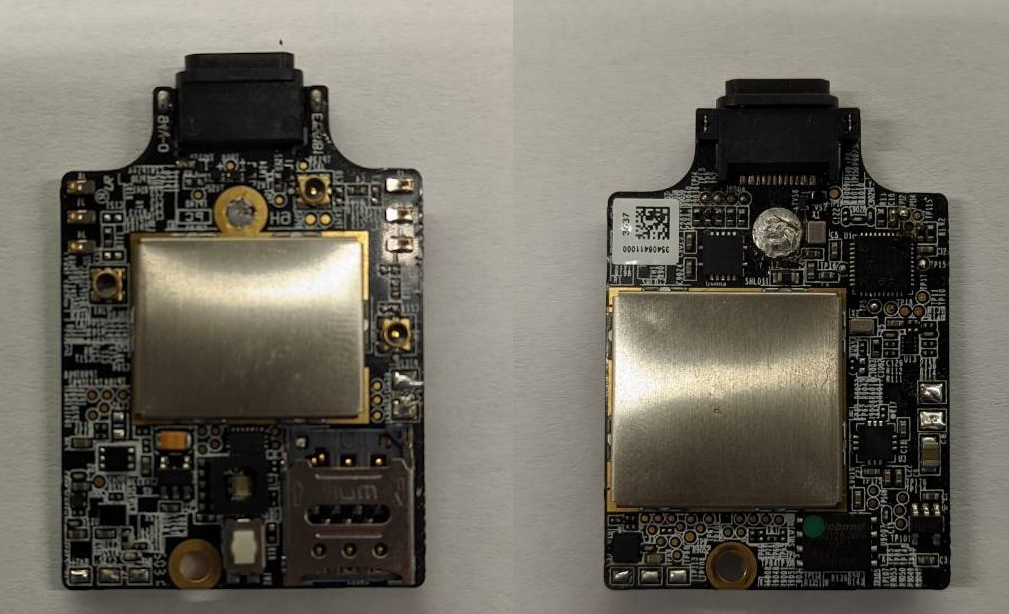
\includegraphics[width=7cm]{Graphics/PCB.png}
    \caption{Wykorzystana płytka PCB z urządzenia dostępnego na rynku}
    \label{img:pcb}
\end{figure}
\section{Podobne rozwiązania obecne na rynku}
Podobne rozwiązanie, zaproponowała firma Specialized. Inżynierowie stworzyli urządzenie o nazwie ANGI, widoczne na rysunku \ref{img:angi_img}. Jest to mały układ, wyposażony w akcelerometr i żyroskop. Komunikuje się on przy użyciu Bluetooth z ich autorską aplikacją na telefon z iOS lub Androidem. Urządzenie, zamontowane na kask, wysyła powiadomienie do aplikacji, gdy rowerzysta uderza kaskiem w przeszkodę. Rozwiązanie to, ma szereg zalet, takich jak prostota budowy i bardzo niskie zużycie energii. Jest ono jednak uzależnione od telefonu, który w przypadku wycieczek górskich, czasem wygodniej zostawić w domu.
\begin{figure}[h]
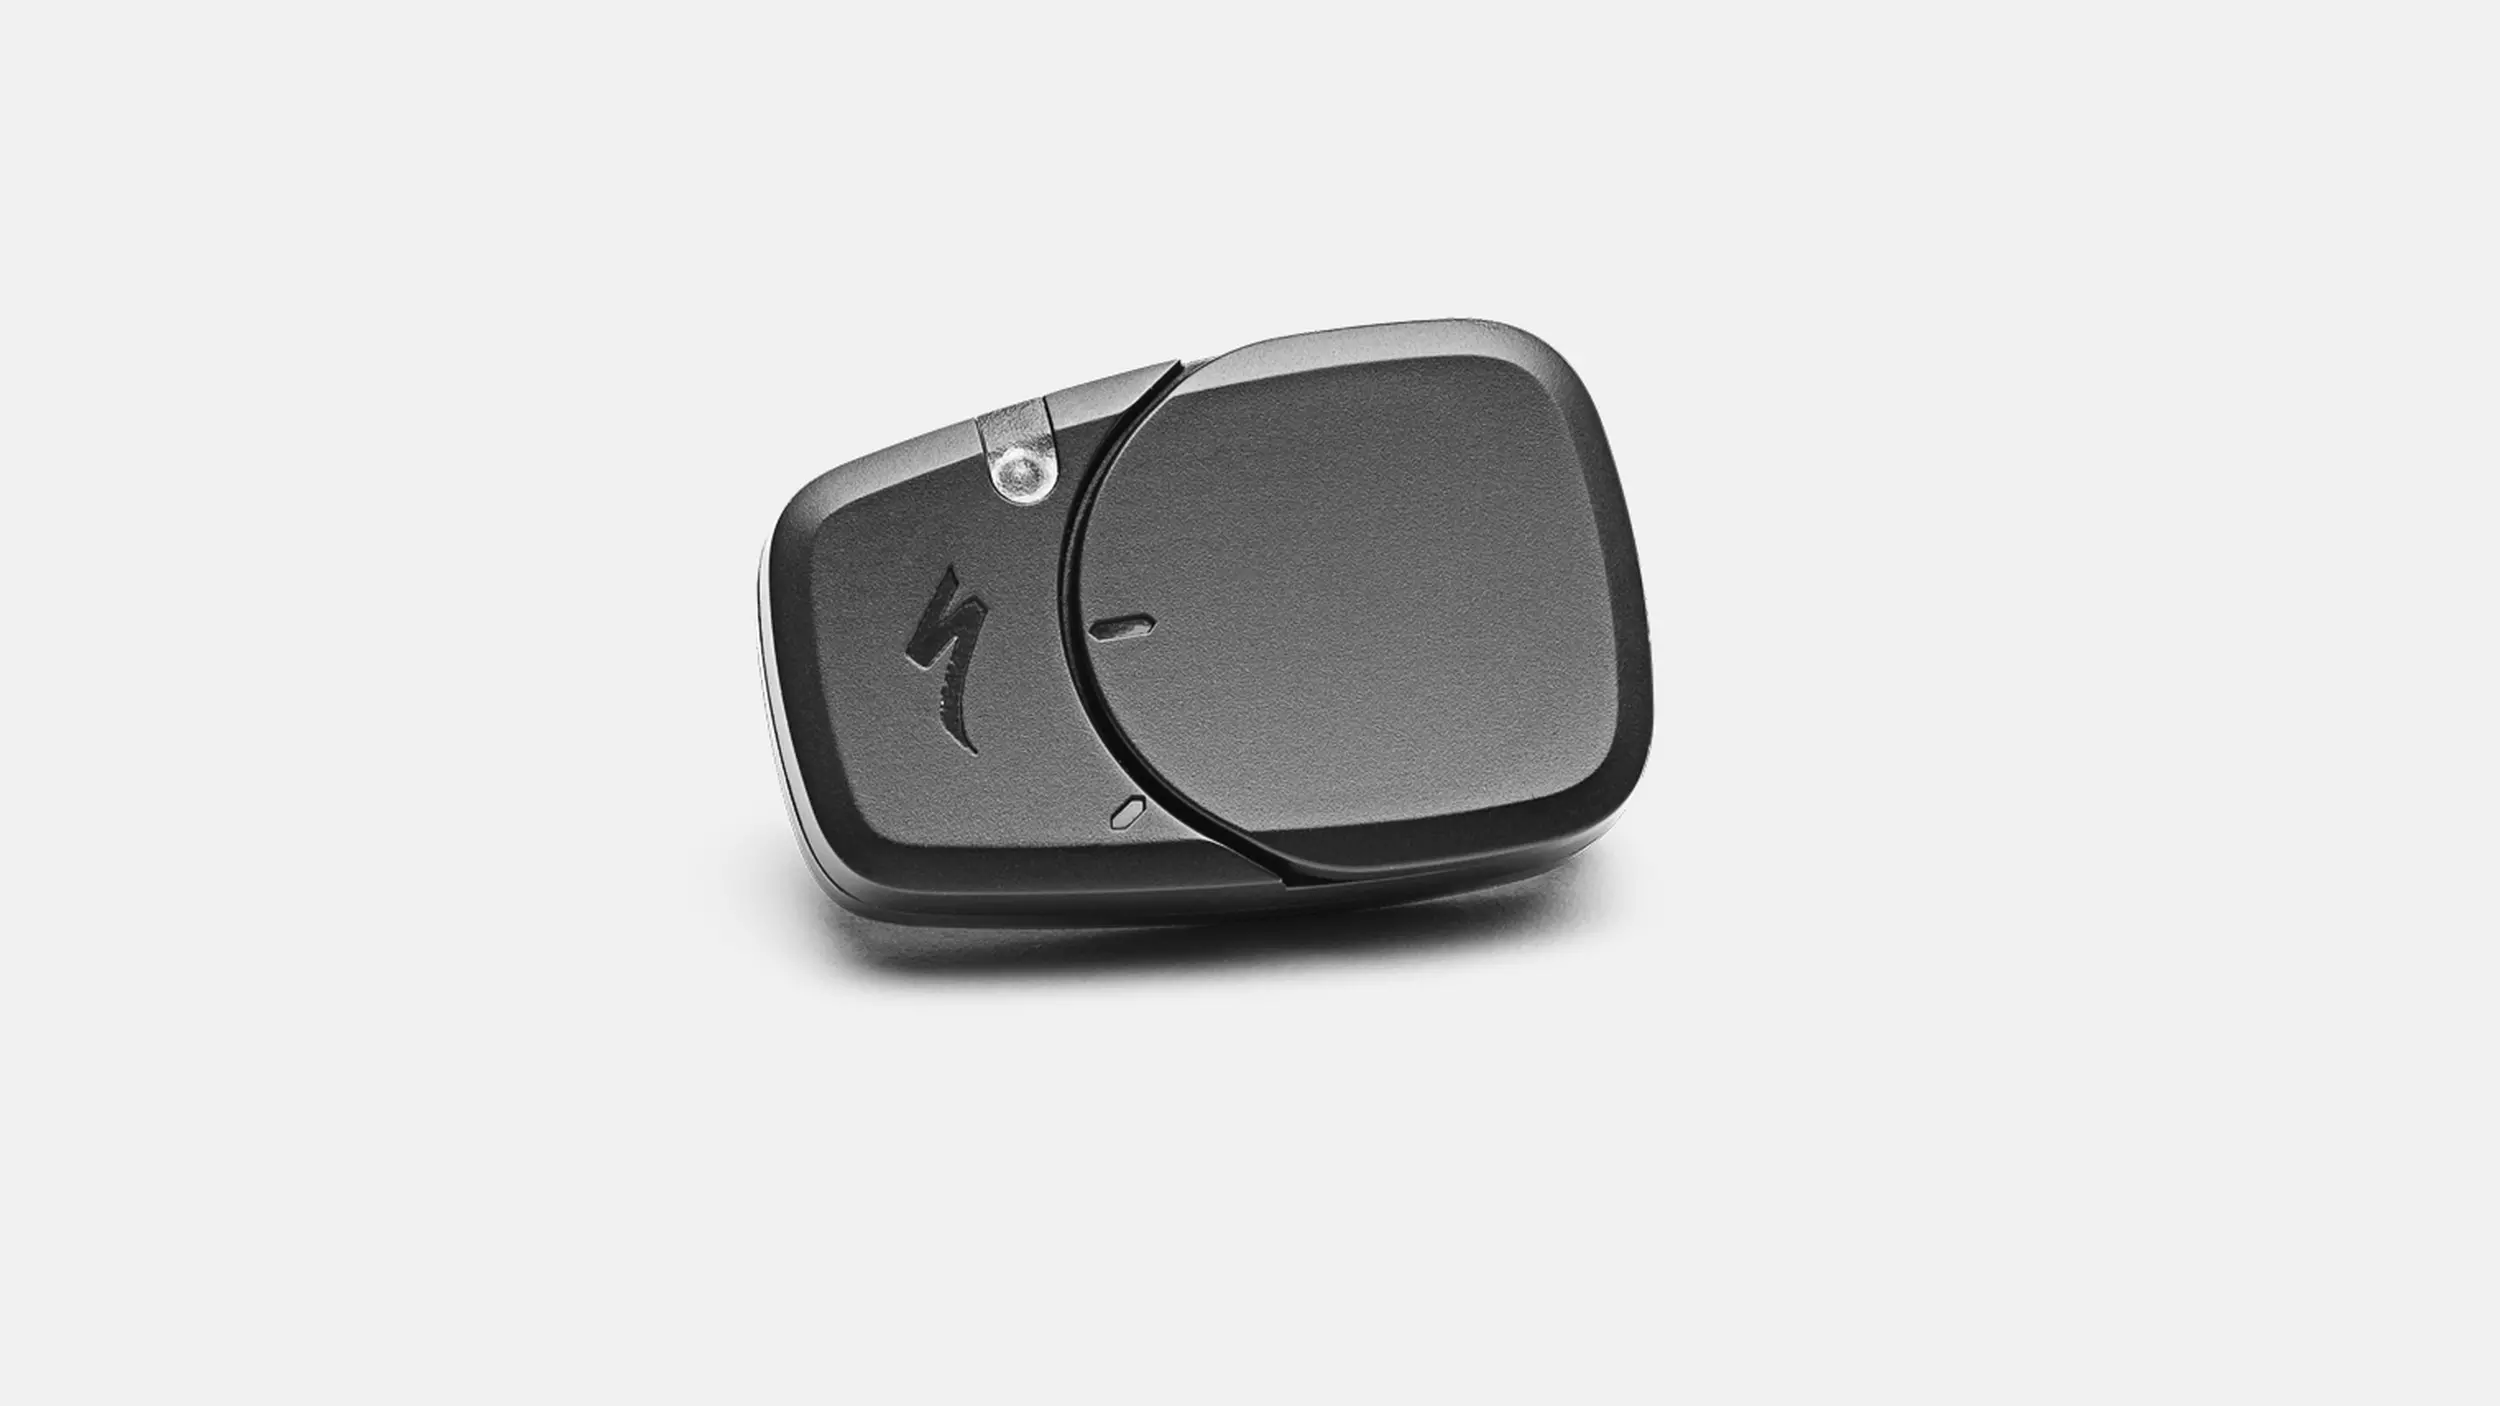
\includegraphics[width=7cm]{Graphics/angi.png}
\centering
\caption{Urządzenie ANGI, stworzone przez firmę Specialized.\cite{ANGI}}
\centering
\label{img:angi_img}
\end{figure}

%---------------------------------------------------------------------------















\chapter{Prototyp urządzenia}
\label{cha:prototyp}

Głównym zagadnieniem pracy było stworzenie kompletnego urządzenia, które wykryje niebezpieczne zdarzenie i poinformuje o tym zdefiniowanego użytkownika. W niniejszym rozdziale, przeprowadzono testy, mające pomóc stworzyć odpowiednie algorytmy. Opisano również kolejne kroki procesu tworzenia urządzenia, a także rozważono różne podejścia w rozwiązaniu problemów. Omówione zostały również poszczególne fragmenty działającego urządzenia.

Tę część pracy, rozpoczęto od przeprowadzenia podstawowych eksperymentów, mających pokazać, jakich przyspieszeń można spodziewać się w przypadku rzeczywistego zderzenia na rowerze. Testy, rozpoczęto od stworzenia urządzenia, mającgo zbierać surowe dane z akcelerometru. Ze względu na łatwość i szybkość implementacji, wykorzystano platformę Raspberry Pi Zero W, z systemem operacyjnym Raspbian Lite. Korzystając z gotowch bibliotek, napisany został skrypt, który po uruchomieniu tworzył plik tekstowy, do którego zapisywał surowe dane, pobrane z akcelerometru. Sam akcelerometr, ustawiony był na częstotliwość próbkowania 416Hz i skalę $\pm$8g.
\newline
Ze względów czysto praktycznych, tj. w celu zabezpieczenia płytek przed uszkodzeniem, wykonany został model 3D prostej obudowy, który następnie wydrukowano na drukarce 3D. Rysunek \ref{img:test_device_a} przedstawia Raspberry w wykonanej na potrzeby projektu obudowie. Zgodnie z rysunkami technicznymi płytki, wykorzystano otwory montażowe. Następnie, stworzono dodatkową warstwę izolacyjną między płytkami, do której przymontowano płytkę z akcelerometrem.(Rysunek \ref{img:test_device_b}) Gotowy układ, zasilany był przy użyciu powerbanku, połączonego przez USB. Obudowa, zamknięta była drukowaną pokrywką. Rozwiązanie przedstawia rysunek \ref{img:test_device_c}.
\newline


\section{Opracowanie algorytmu wykrywania kolizji}
Cały układ, zasilany był przy użyciu zewnętrznej baterii, zamontowanej na siodełku roweru. Ze względu na bezpieczeństwo, testy przeprowadzane były na rowerze bez rowerzysty. Sam układ, zamontowany został na rurze podsiodłowej. Ponieważ jest to prawie centralny punkt roweru, przewidziano, że przyspieszenia w przypadku silnego wyrzucenia koła w powietrze, będą mniejsze. Eksperyment przeprowadzono przez rozpędzanie roweru do  prędkości około 1$\frac{m}{s}$ i kolejno:
\begin{itemize}
    \item Zderzenie roweru z drzewem
    \item Upadek na kamieniach
    \item Upadek ze stromego zbocza
\end{itemize}
%TODO: Podmienić zdjęcie urządzenia testowego
\begin{figure}[h]
    \centering
    \begin{subfigure}{3.5cm}
        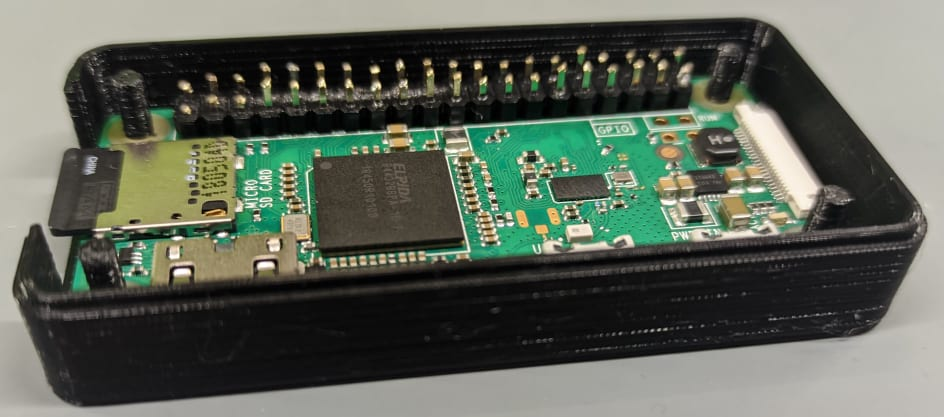
\includegraphics[width=7cm, angle=-90]{Graphics/pi.jpg}
        \caption{Raspberry Pi Zero w drukowanej obudowie}
        \label{img:test_device_a}
    \end{subfigure}
    \begin{subfigure}{3.5cm}
        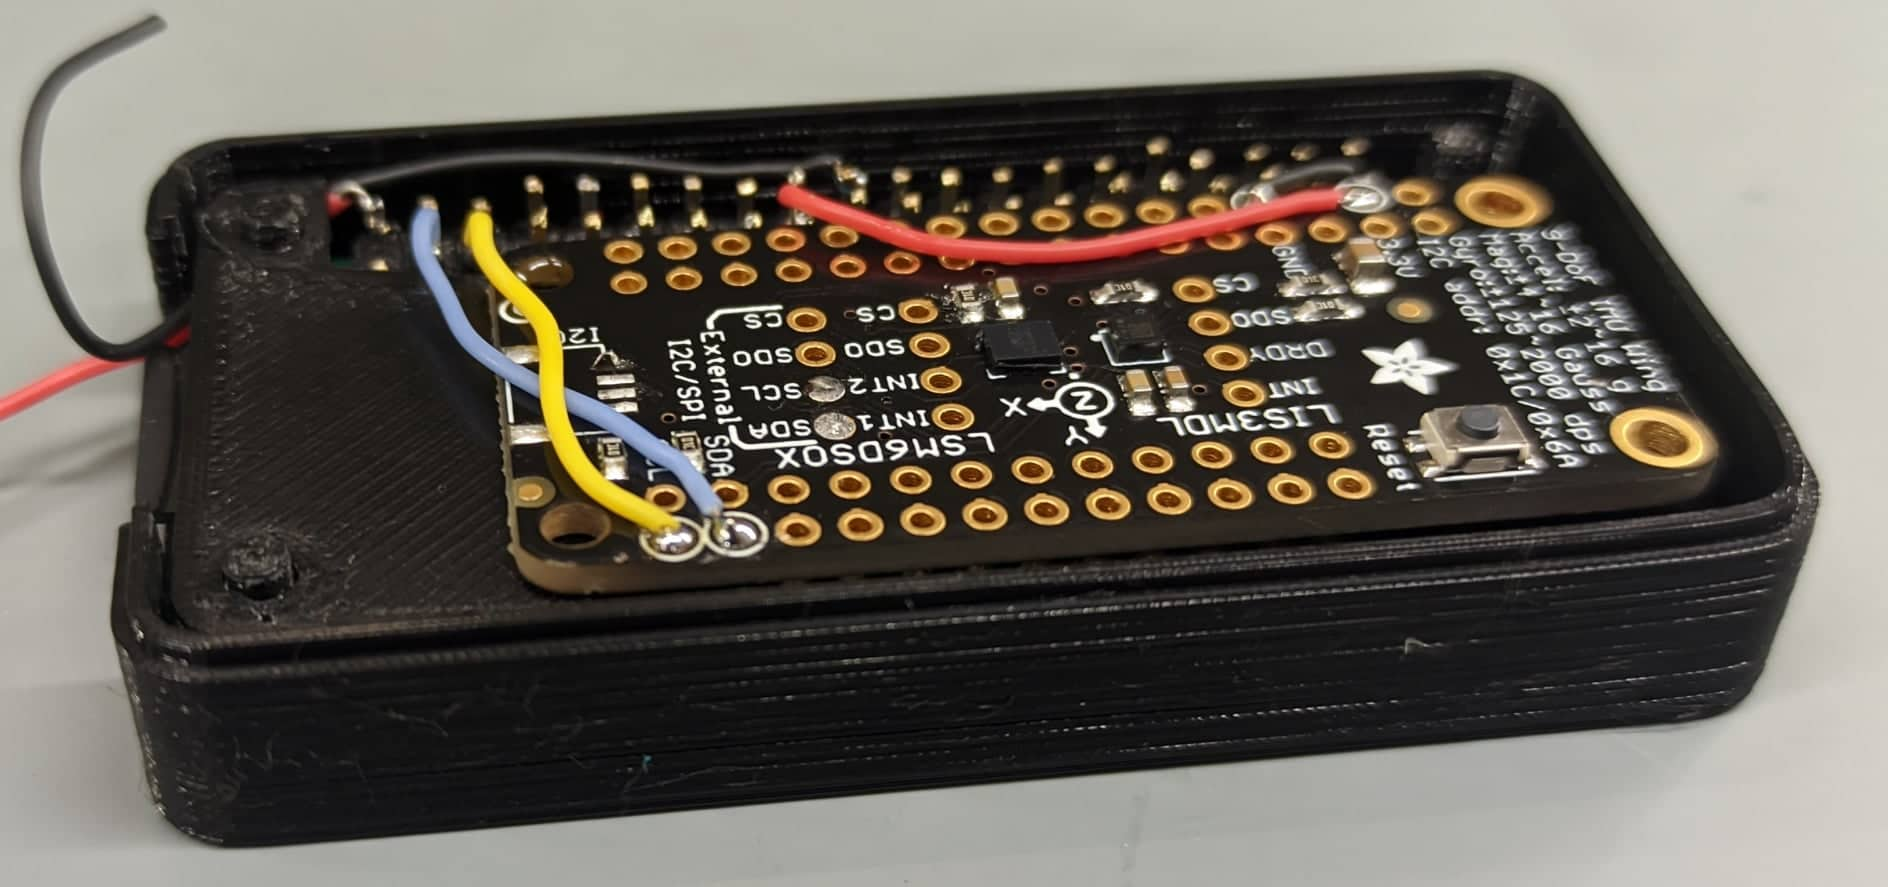
\includegraphics[width=7cm, angle=-90]{Graphics/Pi_acc.jpg}
        \caption{Płytka z akcelerometrem w obudowie}
        \label{img:test_device_b}
    \end{subfigure}
    \begin{subfigure}{3.5cm}
        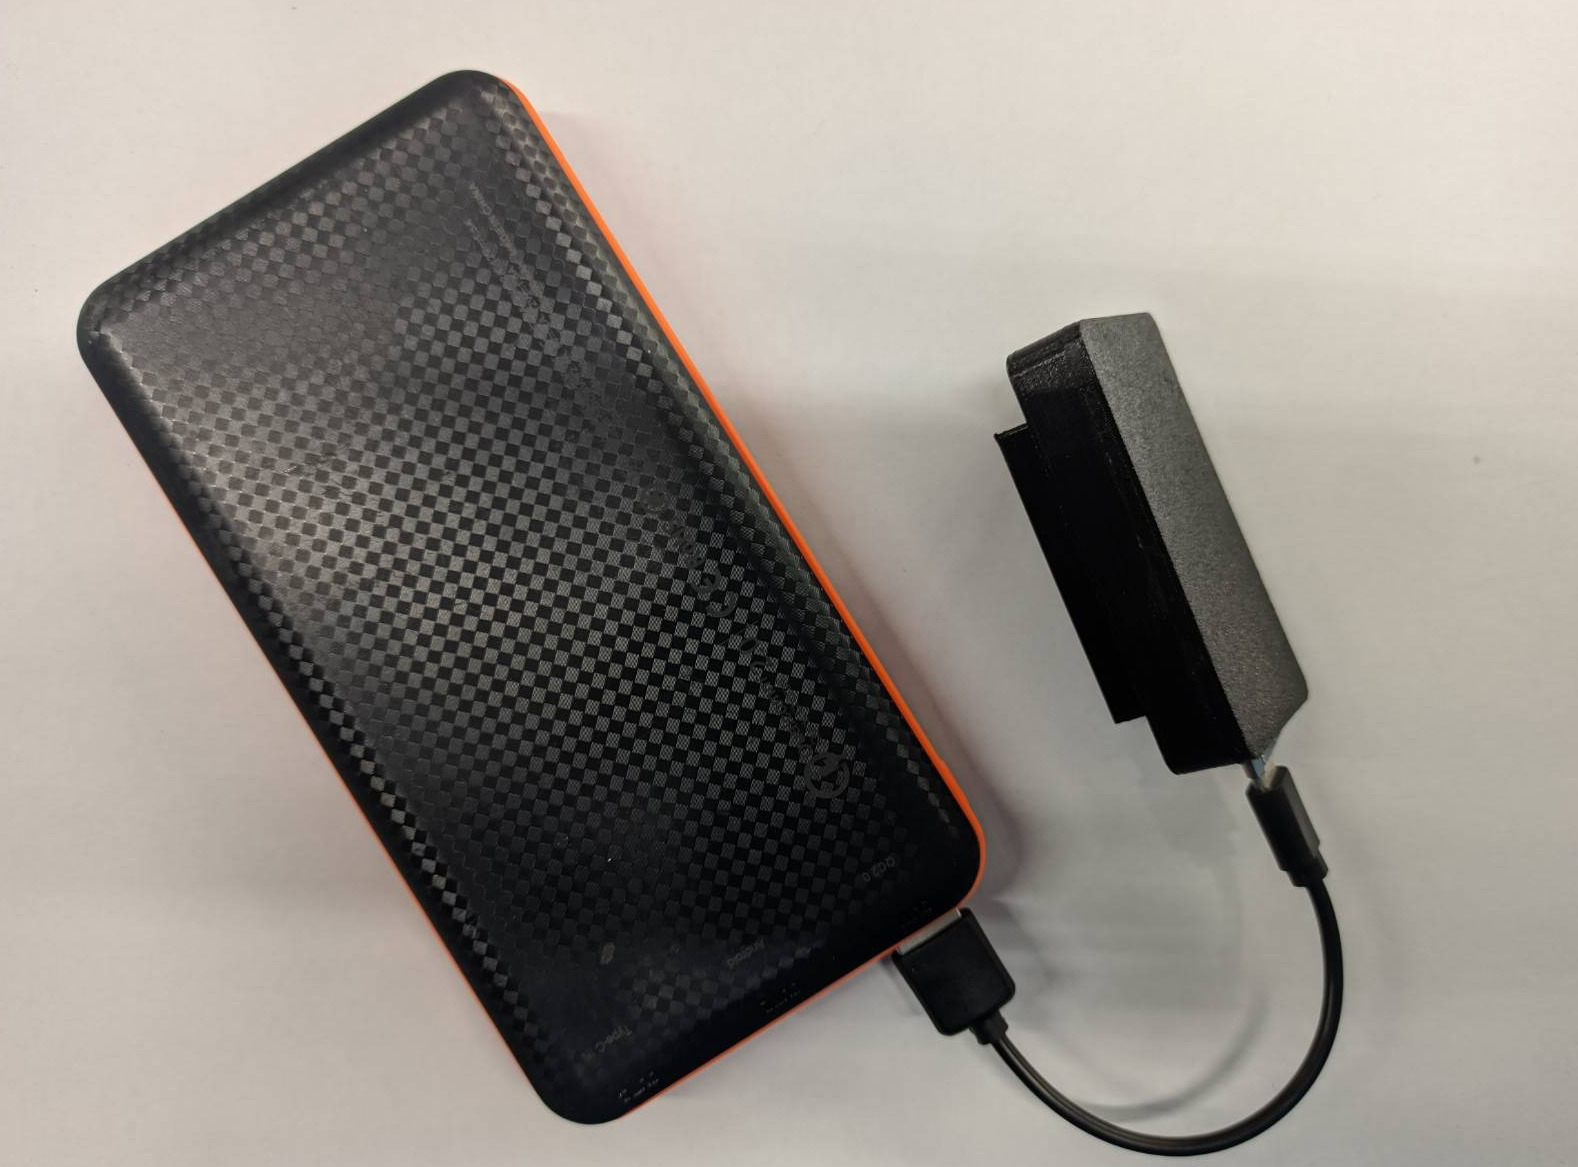
\includegraphics[width=7cm, angle=-90]{Graphics/test_device.jpg}
        \caption{Urządzenie testowe zasilane zewnętrzną baterią}
        \label{img:test_device_c}
    \end{subfigure}
    \caption{Urządzenie testowe do zbierania danych}
\end{figure}

\subsection{Analiza zebranych danych }
\label{sec:data_analysis}
W celu analizy danych, stworzono prosty skrypt w języku Python. Pobierał on surowe dane z pliku, przetwarzał, a następnie rysował zależności czasowe $a(t)$ dla każdej z osi. Ponieważ akcelerometr zwraca liczbę 16-bitową ze znakiem, należało uwzględnić ten fakt w konwersji, gdyż Python posiada dynamiczne typy danych, co mogło zakłamać wyniki. Zebrane dane, okazały się być znacząco zaszumione. Z tego powodu, przefiltrowane zostały filtrem dolnoprzepustowym. Rysunek \ref{img:bike} przedstawia orientację urządzenia na rowerze. W trakcie analizy danych, przyjęto zaznaczone na nim kierunki osi.
\begin{figure}[hb]
    \centering
    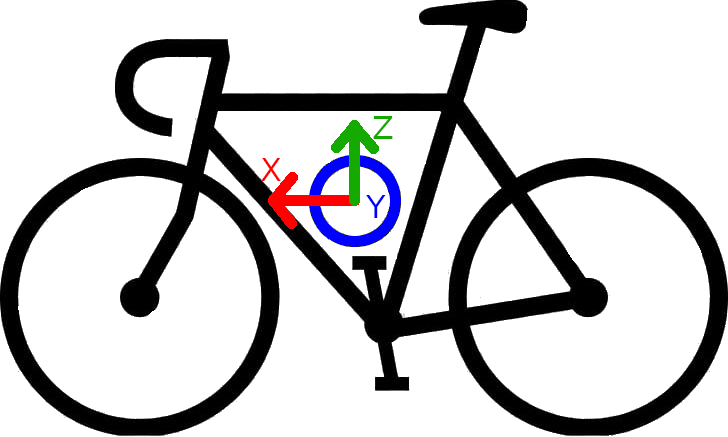
\includegraphics[width=8cm]{Graphics/rowerek.png}
    \caption{Orientacja urządzenia zamontowanego na rowerze}
    \label{img:bike}
\end{figure}
Podczas każdego z testów, rower z przymocowanym urządzeniem, rozpędzono do około 1$\frac{m}{s}$. Zgodnie z przewidywaniami, w większości przypadków przefiltrowane przyspieszenia układu sięgały ok. 1g. Należało również zwrócić uwagę na zwroty przyspieszeń, które zmieniały się po obrocie roweru. Poniżej przedstawiono trzy analizowane przebiegi, na podstawie których utworzone zostały algorytmy. 
\newline
\newline
Rysunek \ref{img:slope} przedstawia zapis upadku ze stromego zbocza. Jest to przypadek gdy rowerzysta górski podczas uskoku, traci kontrolę nad rowerem, lub wypada z trasy. Przez około pół sekundy rower swobodnie spadał, powoli przechylając się w kierunku przedniego koła. Około szóstej sekundy uderzył nim o zbocze, co widać wyraźnie zarówno na osi X, jak i Z. Następnie odbity rower ponownie uderzył w ziemię, tym razem pochylając się po odbiciu na bok. Kolejne uderzenie, było więc uderzeniem bocznym, widocznym jako głęboki dół  na osi Y. Niemal natychmiast, rower obrócił się kołami do góry, co widać na osi Z jako przyspieszenie równe -1g. Po siódmej sekundzie rower zaczął sunąć bokiem wzdłuż zbocza i szybko wyhamowywać. akcelerometr zarejestrował to jako oscylajcje na osi Y pomiędzy 7, a 8 sekundą. Na wykresie, można było również zauważyć, że po zdarzeniu, rower zatrzymał się na jednym z boków, ponieważ oś Y miała stałą wartość bliską 1g.
\newline
\newline
Kolejny z rysunków (\ref{img:stones}), przedstawia sytuację gdy rowerzysta jadąc po kamieniach, uderza tylnym kołem o jeden z nich i traci kontrolę nad rowerem. Sytuacja ta charakterysuje się silnymi oscylacjami osi X i Z, przy względnie stabilnej osi Y. W czwartej sekundzie, rower uderzył tylnym kołem w kamień. Koło zostało wyrzucone do góry, z przyspieszeniem około 1g. Po 500ms rowerzysta rower uderzył z całą energią przednim kołem w ścieżkę, osiągając przyspieszenie prawie 2g. W tej chwili pojazd testowy jeszcze raz odbił się od, a następnie bokiem uderzył w drzewo przy scieżce.
\newline
\newline
Rysunek \ref{img:tree} przedstawia sytuację, gdy rowerzysta tracąc kontrolę nad rowerem, uderza w drzewo. W tym przypadku rower po około 4.5s uderza w drzewo, co odczytane zostało jako wzrost do 0.5g na osi X. Niestety, nie było to uderzenie czyste, ponieważ duża część energii rozłożyła się na odbicie roweru od drzewa. Zapis osi Y pokazuje, że po uderzeniu, rower zaczął obracać się. Ostatecznie jednak, zatrzymał się na jednym z boków.
\newline
\newline
Przeprowadzone testy, pozwoliły na sprawdzenie przeciążeń działających na rower w trakcie wypadku. Pierwszym z nasuwających się wniosków był fakt, że niepotrzebnie ograniczona została częstotliwość próbkowania akcelerometru. W przypadku Raspberry Pi, magistrala I$^{2}$C, pozwala na transmisję 12,5kB/s. Ponieważ jeden zestaw danych zawierał 12 bajtów, częstotliwość próbkowania mogła wynosić aż 1kHz. Tymczasem, ustawiona została częstotliwość 416Hz. Ustawienie to wynikało z obawy, że kod w języku skryptowym nie nadąży za większą częstotliwością. Kolejnym z wniosków, była konieczność stosowania filtrów dolnoprzepustowych. Surowe zapisy z akcelerometru, były silnie zaszumione, na co również wpływ mogła mieć mała częstotliwość próbkowania względem szybkości zmian podczas wypadku. Mimo tego, testy dostarczyły cennych danych na podstawie których stworzono algorytmy, opisane w podrozdziale \ref{sec:state_machines}

%%%%%%%%% Zapisy upadku - wykresy %%%%%%%%%%
\begin{figure}[H]
    \centering
    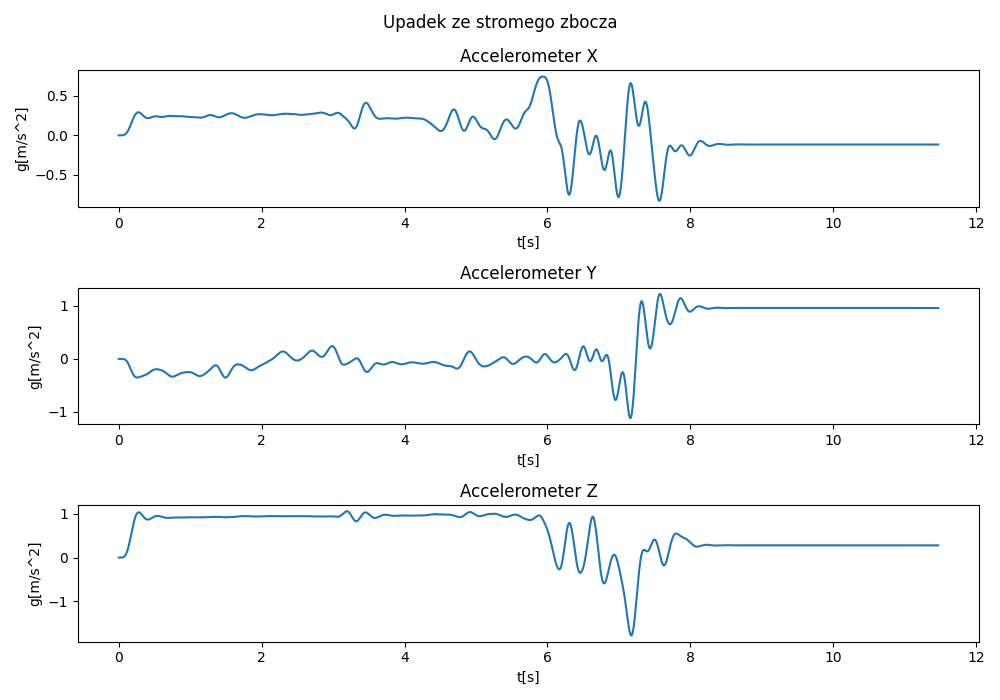
\includegraphics[width=15cm]{Graphics/slope_title.png}
    \caption{Przefiltrowany zapis upadku roweru ze stromego zbocza}
    \label{img:slope}
    \vspace{0.5cm}
    \centering
    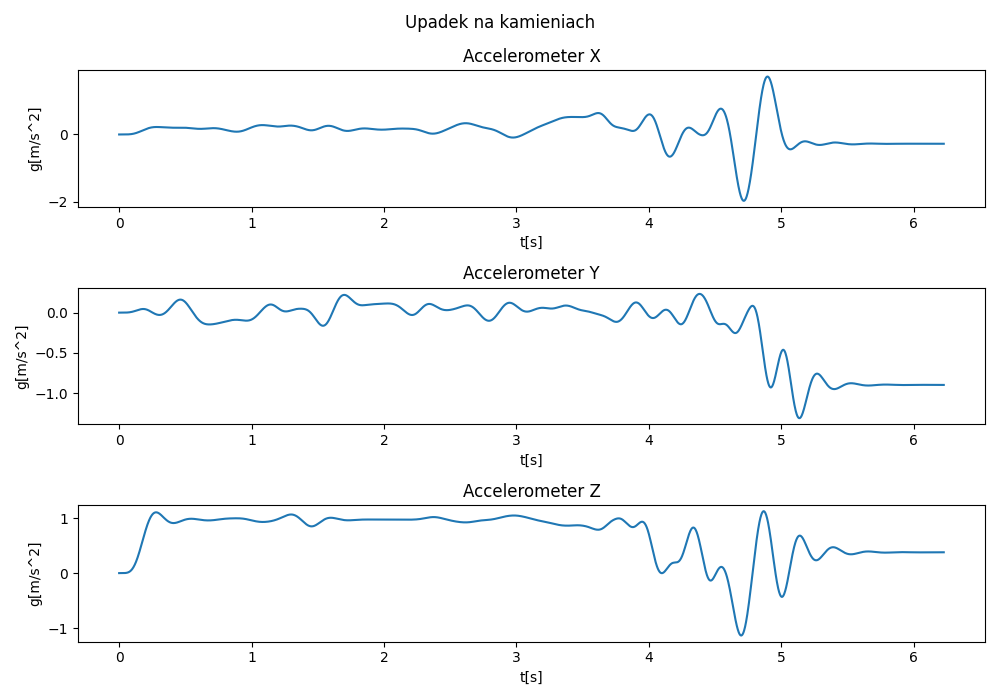
\includegraphics[width=15cm]{Graphics/Stones_title.png}
    \caption{Przefiltrowany zapis upadku roweru na kamieniach}
    \label{img:stones}
\end{figure}
\begin{figure}[h]
    \centering
    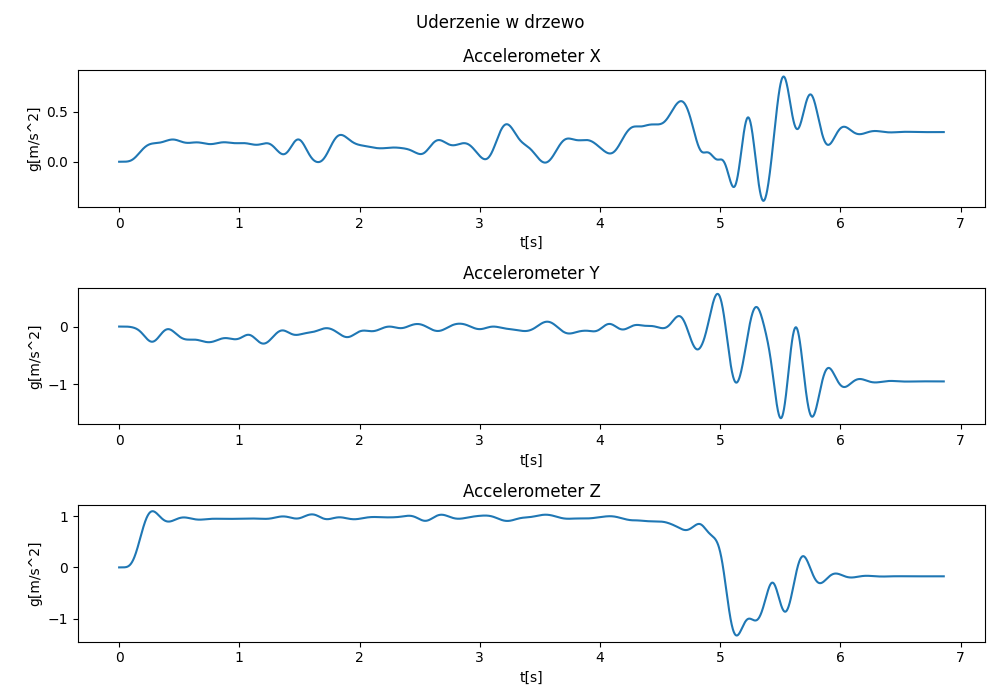
\includegraphics[width=15cm]{Graphics/Tree_title.png}
    \caption{Przefiltrowany zapis uderzenia roweru w drzewo}
    \label{img:tree}
\end{figure}

\subsection{Maszyny stanów wykrywające wypadek}
\label{sec:state_machines}
Na podstawie analizy danych z podrozdziału \ref{sec:data_analysis} zdecydowano się na implementację czterech, niezależnych maszyn stanów. Każda z nich, odpowidać będzie analizowanym przypadkom. Istotnym elementem pracy było możliwie największe uproszczenie maszyn, aby przyspieszyć działanie układu i zminimalizować zużycie energii, bez utraty skuteczności.
\subsubsection{Wykrywanie przeciążenia w dowolnej osi}
Pierwsza z maszyn stanów, służy wykryciu znaczących przeciążeń na dowolnej z osi. Podczas testów zauważono, że podczas każdego z wydarzeń, wysoka wartość przeciążenia odróżnialna była od szumu na podstawie czasu trwania. Określono, że jeśli po około 50ms próbka utrzymuje wysoką wartość, to nastąpiło silne przeciążenie. Ponieważ zdecydowano się skorzystać z wbudowanych w akcelerometr maszyn stanów, można było skorzystać z ich wewnętrznych liczników. Opisywana maszyna stanów, gdy dowolna z osi przekroczy wartość $\pm$6g, ustawia licznik na 50ms. Gdy przez ten czas, nie wystąpi próbka o wartości mniejszej niż 6g, wyzwolony zostaje alarm. Duża wartość przyspieszenia, pozwoliła uniknąć fałszywych alarmów podczas bezkolizyjnej jazdy. Maszynę przedstawia diagram \ref{img:fsm1}.
\newline
\newline
\subsubsection{Maszyna stanów wykrywająca przewrócony rower}
Dwie kolejne maszyny stanów, przedstawione na diagramie \ref{img:fsm2}, to algorytmy wykrywające przewrócenie roweru. Podczas analizy danych zauważono, że każdy wypadek, kończył się przechyleniem roweru na jeden z boków. Z tego powodu, zaimplementowano licznik, który co 2 sekundy próbkuje wartość na osi Y i sprawdza, czy przekroczyła ona wartość bezwzględną 0.6g. Jeśli przez dwie minuty, rower nie wróci do pozycji jazdy (|Y| < 0.6g), wyzwolony zostaje alarm. W praktyce, opisana maszyna musiała zostać zaimplementowana w akcelerometrze jako dwie, niezależne, z uwagi na brak funkcji wartości bezwzględnej w układzie.
\begin{figure}[h]
    \centering
    \begin{subfigure}[b]{5cm}
    \centering
    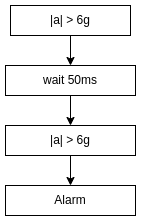
\includegraphics[width=3.5cm]{Graphics/All_axis_FSM1.png}
    \caption{Wykrycie silnego przeciążenia}
    \label{img:fsm1}
    \end{subfigure}%
    \hspace{1cm}
    \begin{subfigure}[b]{5cm}
    \centering
    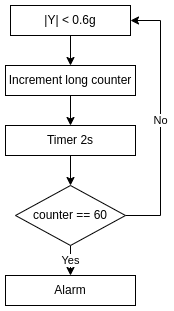
\includegraphics[width=4cm]{Graphics/overturned_FSM2_3.png}
    \caption{Wykrycie przewrócenia roweru}
    \label{img:fsm2}
    \end{subfigure}
    \caption{Maszyny 1-3}
\end{figure}
\subsubsection{Maszyna stanów wykrywająca uderzenie i upadek}
Ostatnia z maszyn stanów (rysunek \ref{img:fsm4}), wykrywa uderzenie w osi Z, czyli np. najechanie na korzeń. Następnie, przez 60 sekund sprawdza, czy rower nie wrócił do wyjściowej pozycji, czyli zwykłej jazdy. W przypadku, gdy przez 10 sekund rower nie powróci do pionu, uruchomiony zostanie alarm. Maszyna ta, okazała się być najdokładniejszą z prezentowanych. Wynika to bezpośrednioz faktu, że oś Z jest osią najbardziej stabilną w trakcie jazdy. Pozostałe maszyny, stanowią więc jej uzupełnienie.
\begin{figure}[h]
    \centering
    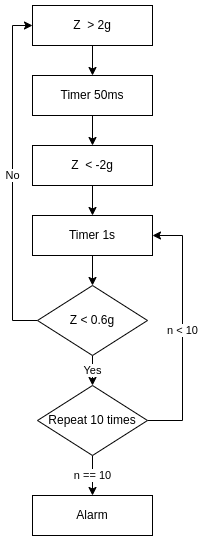
\includegraphics[width=4cm]{Graphics/Z_axis_FSM.png}
    \caption{Czwarta maszyna stanów}
    \label{img:fsm4}
\end{figure}

\section{Opracowanie logiki urządzenia}

\subsection{Wysokopoziomowy algorytm działania urządzenia}
Głównym zagadnieniem budowy urządzenia, było maksymalne wydłużenie czasu pracy na baterii. Z tego powodu, założono, że lokalizacja oraz połączenie z siecią, będą zestawiane tylko w momencie wystąpienia wypadku. Na podstawie rozważań oraz testów przeprowadzonych w podrozdziale \ref{sub:recognize-choice}, zdecydowano się na wykorzystanie maszyny stanów wbudowanej w akcelerometr. Dzięki temu, możliwym było ustawienie urządzenia w tryb głębokiego uśpienia, tuż po inicjalizacji urządzenia.
Rysunek \ref{img:app_logic} obrazuje założoną logikę urządzenia. Po uruchomieniu układu, inicjalizowane są wszystkie komponenty. W przypadku LTE, wykonywana jest rejestracja do sieci. Ponieważ jest to urządzenie odpowiedzialne za bezpieczeńswo, rejestracja przy uruchomieniu może wykryć nieprawidłowości jak brak środków na koncie, brak karty SIM czy urwana antena modemu. Ta funkcjonalność, nie została jednak zaimplementowana na tym etapie rozwoju urządzenia. Po inicjalizacji podzespołów, wyłączony został zarówno modem oraz moduł GPS. Zgodnie z założeniami, są one uruchamiane w momencie wystąpienia alarmu, aby oszczędzić energię. Kolejnym krokiem, jest wgranie zrzutu pamięci akcelerometru, celem ustawienia maszyn stanów. Po jego wykonaniu, mikrokontroler przechodzi w tryb uśpienia. W tle, uruchomiony pozostaje stos Bluetooth, pozwalając połączyć się z urządzeniem i wpisać numer telefonu, na który wysłane zostanie powiadomienie. Wyzwolenie dowolnej z maszyn stanów, uruchamia przerwanie. Wyzwolenie przerwania, skutkuje uruchomieniem modułu GPS, a po poprawnym pobraniu lokalizacji, również modemu. Powiadomienie, jest wysyłane periodycznie, do momentu wyłączenia alarmu przyciskiem. Pomiędzy alarmami, wszystkie podzespoły pozostają wyłączone, celem oszczędzania anergii.
\begin{figure}[h]
    \centering
    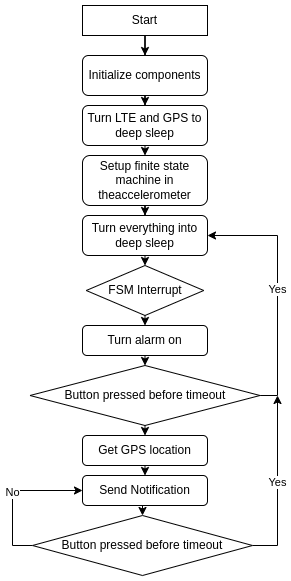
\includegraphics[width=6cm]{Graphics/APP_logic.png}
    \caption{Diagram przedstawiający logikę działania urządzenia}
    \label{img:app_logic}
\end{figure}
%%%%% Accel %%%%%
\subsection{Wybór metody analizy danych przez urządzenie}
\label{sub:recognize-choice}
Ponieważ jednym z najważniejszych elementów pracy, było osiągniecie jak najniższego zużycia energii, zdecydowano się na porównanie podejścia klasycznego, opartego na czytaniu danych i ich analizie przez mikrokontroler, z maszynami stanów realizowanymi przez akcelerometr. W tym celu, skonfigurowano prosty algorytm, wykrywający obrót urządzenia w osi Z. Akcelerometr ustawiono w tryb niskiego zużycia energii, a następnie wprowadzono mikrokontroler w tryb uśpienia. W tym stanie, układ oczekiwał na przerwanie, informujące o gotowości danych. Po jego wystąpieniu, następowało zczytanie danych z akcelerometru, a następnie porównanie ich do zdefiniowanej stałej. Po spełnieniu warunku obrotu o 180$^{\circ}$, ustawiano licznik na 2 sekundy, resetujący stan maszyny. Jeśli w tym czasie, odczytano dane o przeciwnym znaku, maszyna stanów uznana była za zrealizowaną, o czym informowano przez wiadomość wypisaną na UART. Całość, zobrazowana jest na diagramie \ref{img:recognize}.

\begin{figure}[h]
    \centering

    \begin{subfigure}[b]{5cm}
    \centering
    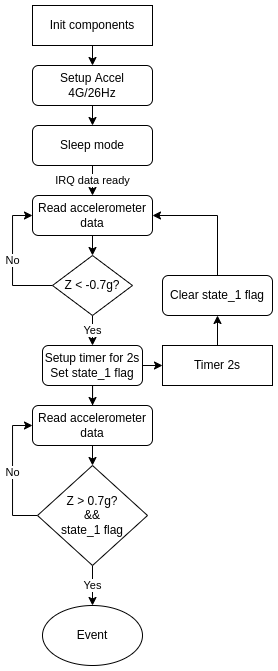
\includegraphics[width=5cm]{Graphics/Recognize_in_code.png}
    \caption{Wykrywanie zdarzenia przez mikrokontroler}
    \end{subfigure}%
    \hspace{3cm}
    \begin{subfigure}[b]{5cm}
    \centering
    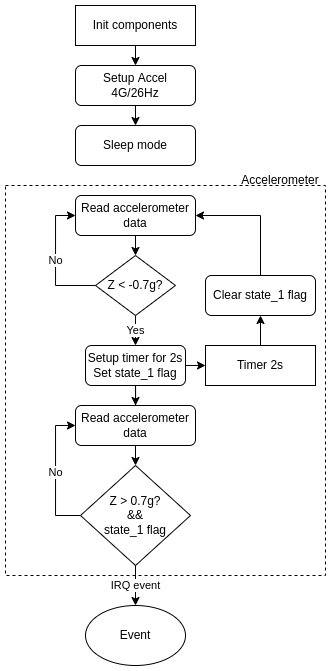
\includegraphics[width=5cm]{Graphics/Recognize_in_code_acc.png}
    \caption{Wykrywanie zdarzenia przez akcelerometr}
    \end{subfigure}%
    \caption{Analiza zdarzenia przez mikrokotroler lub akcelerometr}
    \label{img:recognize}
\end{figure}
Każde rozwiązań, zostało zmierzone przy użyciu urządzenia Otii. Jest to urządzenie służące do precyzyjnej analizy energii pobieranej przez układ \cite{otii}. Na zapisie z programu(rys. \ref{img:recognize_mcu}) wyraźnie widać inicjalizację modemu LTE, który w trakcie przeprowadzania testów był już zintegrowany na płyce PCB. Jest ona widoczna w postaci znaczącego wzrostu pobieranego przez układ prądu, sięgającego nawet 200mA. Gdy modem przechodzi w tryb głębokiego uśpienia, wyraźnie widać odczyty i przerwania, w postaci drobnych pików. Sam skok, wynikał z wywołania funkcji logującej, jednak w wyraźny sposób zaznaczał moment wystąpienia przerwania. W przypadku tego podejścia, pobór prądu wyniósł 1.58mA. Należy jednak zaznaczyć, że zastosowana tutaj maszyna stanów, była maszyną bardzo prostą. Jej rozbudowa, wiązałaby się z bardzo szybkim wzrostem zużycia energii. Kolenym z minusów była ilość generowanych przez akcelerometr przerwań. Każdy odczyt danych nie tylko zajmuje linię danych I$^{2}$C, ale również czas procesora. 
\begin{figure}[h]
    \centering
    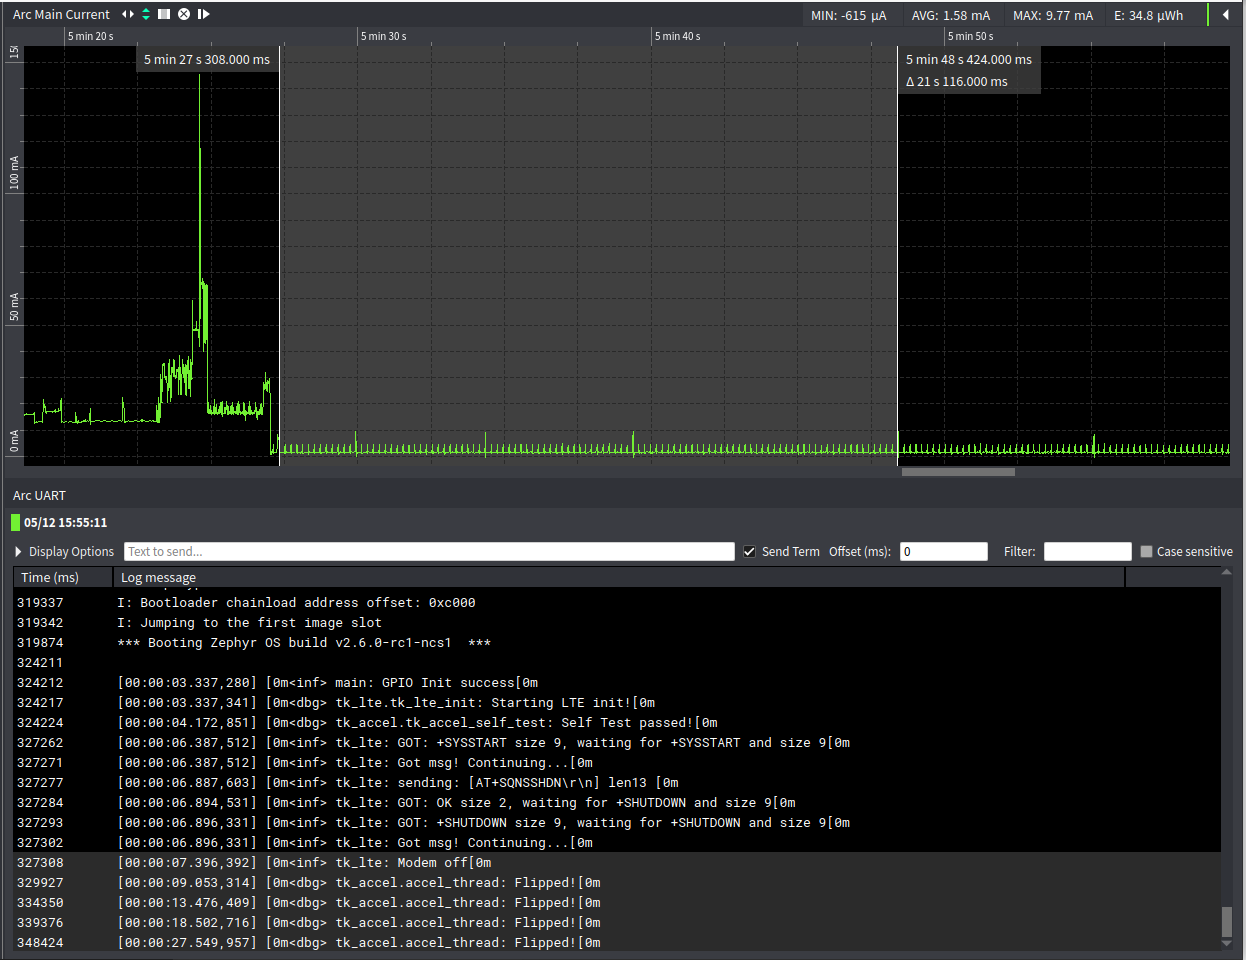
\includegraphics[width=15cm]{Graphics/recognize_mcu.png}
    \caption{Pobór prądu w czasie, podczas analizy przez mikrokontroler}
    \label{img:recognize_mcu}
\end{figure}
\newline
Podejście drugie, z maszyną stanów skonfigurowaną na akcelerometrze, okazało się zużywać średnio aż o 200$\mu$A mniej. Tak duża różnica, przy tak prostej funkcjonalności, była silnym argumentem za wykorzystaniem wbudowanej maszyny stanów. Dodatkowo, na rysunku \ref{img:recognize_acc} widać, że zniknęły gęste piki prądu. Wynikało to wprost z tego, że akcelerometr wystawia przerwanie tylko wtedy, gdy spełniona wykonana zostanie cała maszyna stanów.
\begin{figure}[h]
    \centering
    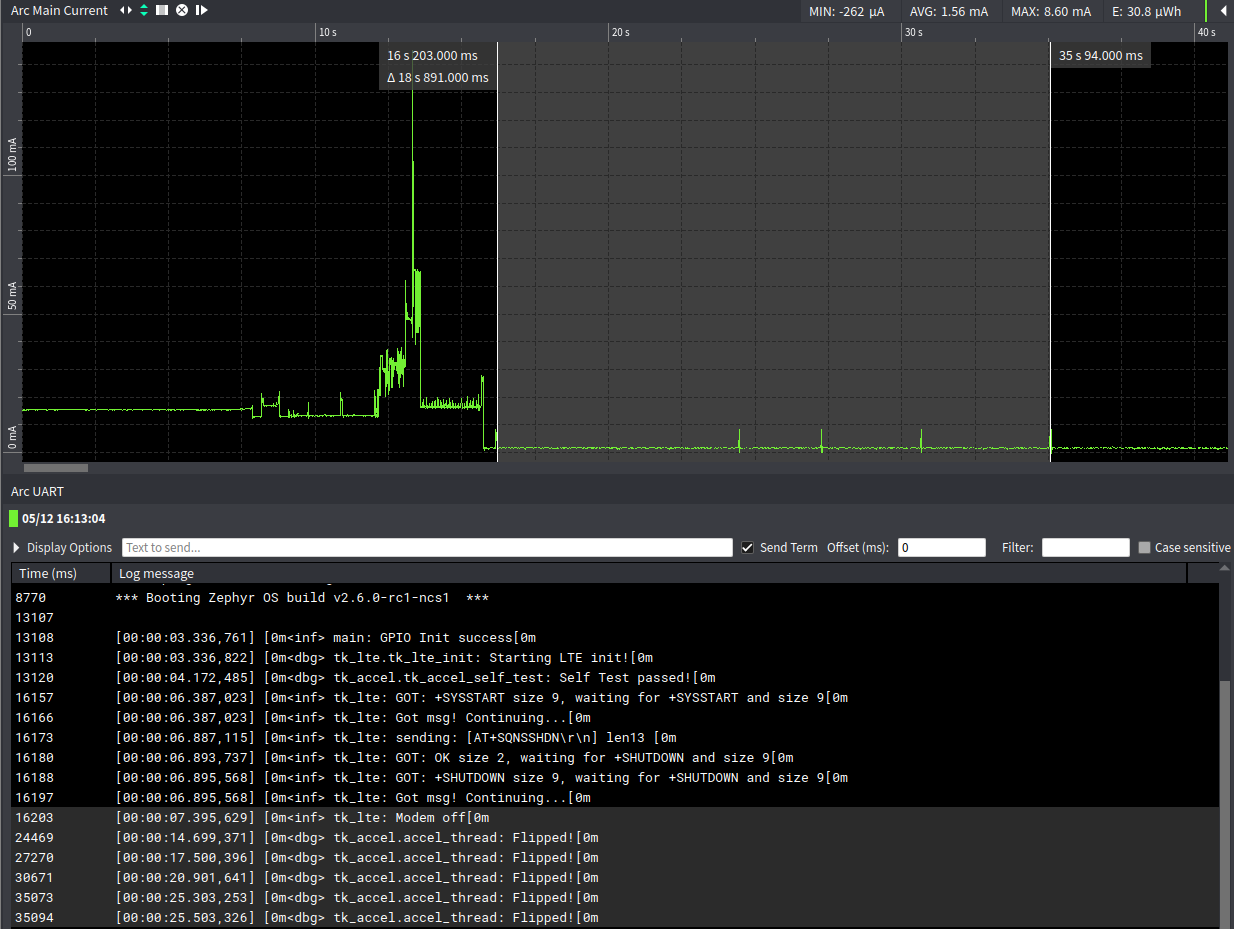
\includegraphics[width=15cm]{Graphics/recognize_acc.png}
    \caption{Pobór prądu w czasie, podczas analizy przez akcelerometr}
    \label{img:recognize_acc}
\end{figure}
Powyższe rozważanie, pokazało więc zasadność stosowania akcelerometru analizującego dane niezależnie od mikrokontrolera. Dodatkowo, STMelectronics, stworzyło zestaw narzędzi, ułatwiających budowę urządzeń, w oparciu o ich układy. Przykładem jest program Unico-GUI\cite{unico}, pozwalający programować akcelerometry w oparciu o płytki rozwojowe. Podczas tworzenia tej pracy, wykorzystano zestaw STEVAL-MKI109V3 + STEVAL-MKI197V1. Program Unico, pozwala projektować maszyny stanów w oparciu o interfejs graficzny. Było to znaczące ułatwienie, ze względu na możliwość zapisania zrzutu pamięci akcelerometru do kodu w języku C. Dzięki temu, w łatwy sposób można było testować różne konfiguracje układu, unikając ręcznego nadpisywania rejestrów. Pomocną okazała się również nota aplikacyjna, wyjaśniająca sposób, w jaki maszyny stanów powinny być programowane \cite{lsm6dsoxappnote}. Na rysunku \ref{img:unico_ss} pokazano zrzut programu, przedstawiąjący ustawienie maszyny stanów numer 1.
\begin{figure}[h]
    \centering
    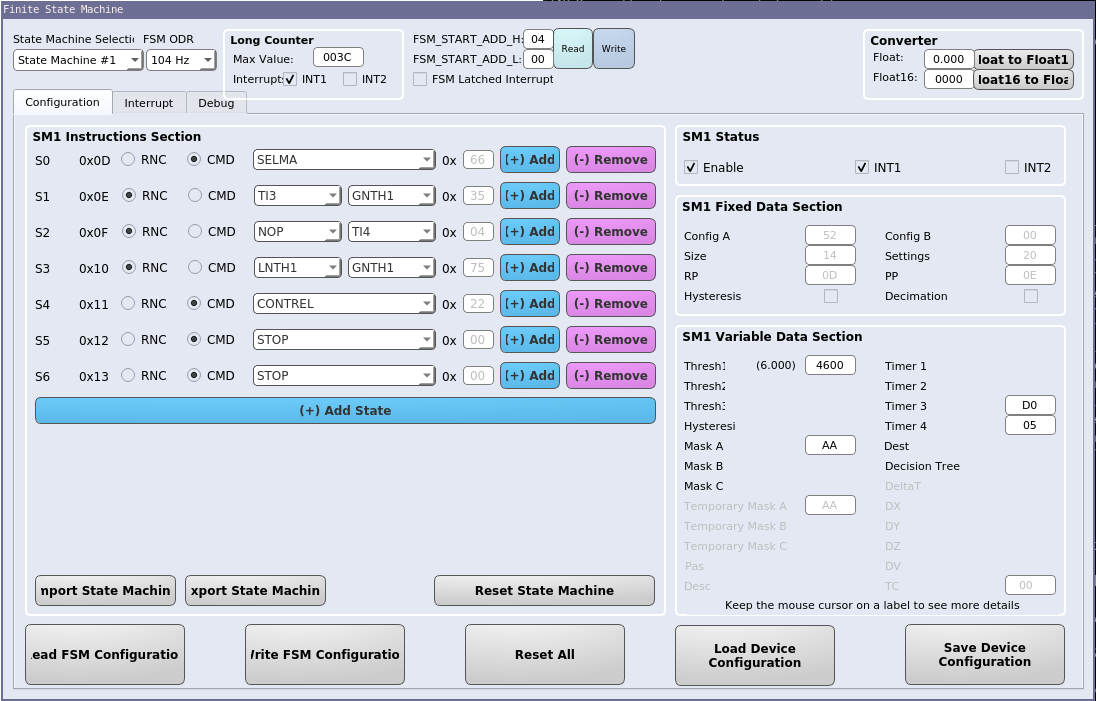
\includegraphics[width=12cm]{Graphics/unico_screenshot.png}
    \caption{Zrzut programu Unico-GUI. Implementacja maszyny stanów numer 1}
    \label{img:unico_ss}
\end{figure}
%%%%% GPS %%%%%
\subsection{Implementacja pobierania lokalizacji}
Zasada działania modułu MT3333 jest stosunkowo prosta. Zgodnie z dokumentacją\cite{MT3333}, należało w odpowiedniej kolejności uruchomić przetwornice układu, zachowując właściwe odstępy czasowe. Gdy zostaną one uruchomione poprawnie, układ zacznie szukać lokalizacji, jednocześnie cały czas wysyłając wiadomości NMEA. Wyzwaniem okazało się tutaj parsowanie przychodzących wiadomości. Ostatecznie, do bufora dopisywane były bajty, do momentu otrzymania znaku nowej linii. Przychodzące linie były testowane przez algorytm. Po otrzymaniu wiadomości zawierającej lokalizację, wiadomość parsowana była do struktury, zawierającej szerokość i wysokość geograficzną w postaci tablic bajtów. Po otrzymaniu lokalizacji, moduł był wyłączany, aby nie marnować energii. Schemat działania, przedstawiono na diagramie \ref{img:gps_diagram}.
\begin{figure}[h]
    \centering
    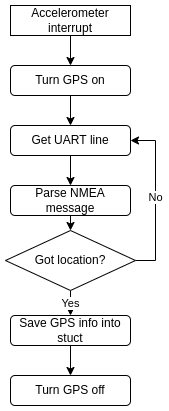
\includegraphics[width=4cm]{Graphics/GPS_NMEA.png}
    \caption{Działanie modułu GPS}
    \label{img:gps_diagram}
\end{figure}

%%%%% LTE %%%%%
\subsection{Implementacja powiadamiania o zdarzeniu}
Dzięki zastosowaniu układu SKY66430, podczas tworzenia prototypu, przetestowano dwa, zupełnie różne podejścia do problemu powiadamiania:
\begin{itemize}
    \item Zapytanie HTTP
    \item Powiadomienie SMS
\end{itemize}
Każde z podejść, zakładało logikę, przedstawioną na rysunku \ref{img:lte_diagram}. Całość komunikacji z modemem, realizowana była przy użyciu komend AT. Ważnym problemem, była kolejność wysyłanych do niego poleceń. Z tego powodu, zaimplementowana została funkcja oczekująca na odpowiedź od modemu, potwierdzającą przetworzenie wysłanej komendy. Dzięki jej zastosowaniu, zminimalizowana została szansa niepowodzenia transmisji, ponieważ w przypadku zbyt długiego oczekiwania, modem był resetowany przeznaczonym do tego pinem.
\begin{figure}[t]
    \centering
    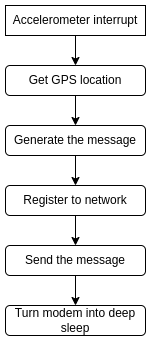
\includegraphics[width=4cm]{Graphics/LTE.png}
    \caption{Procedura wysłania powiadomienia o zdarzeniu}
    \label{img:lte_diagram}
\end{figure}

Na potrzeby przetestowania zapytań HTTP, stworzone zostało proste gniazdo TCP w JavaScript. Następnie, wykorzystując gotowe biblioteki, zaprogramowano bota na platformę Discord. Jest to platforma oparta o otwarty kod źródłowy, na której użytkownicy tworząc kanały głosowe i tekstowe, komunikują się w zorganizowany sposób. Bot, jest wirtualnym użytkownikiem, wykonującym zaprogramowane akcje. Mogą one obsługiwać specjalne funkcje serwera, lub monitorować zachowanie użytkowników. W omawianym podejściu, bot mógł wysłać powiadomienie z otrzymaną lokalizacją, do wszystkich użytkowników serwera. Ponieważ platforma posiada bardzo dobrze rozwiniętą aplikację mobilną, powiadomienie mogłoby być szybko odczytane przez jednego z użytkowników. Jednocześnie, nie byłoby wymagane definiowanie jednego, numeru docelowego. Ostatecznie jednak, rozwiązanie to zostało uznane za niepasujące do urządzenia na tym etapie. Takie podejście, wymagało stworzenia stabilnego kodu zewnętrznej aplikacji (bota). Jednocześnie, zapytanie HTTP przesyła dużo danych, w porównaniu do SMS. Mogło to okazać się problemem w miejscach o słabym zasięgu.
\newline
Finalnie, zdecydowano się na wysłanie prostego powiadomienia tekstowego, przy użyciu wiadomości SMS. Za tym rozwiązaniem, przemawiała stabilność i niezawodność sieci komórkowych, mających obecnie niemal całkowite pokrycie, nawet w górach. Wysłanie SMS, pozwoliło również uniezależnić urządzenie od innych aplikacji.
Ponieważ współrzędne geograficzne, nie są szczególnie użyteczne bez mapy, wysyłane powiadomienie SMS zawiera zawiera link do map Google. Link ten jest tworzony w kodzie układu, wykorzystując funkcje bibliotek standardowych. Rysunek \ref{img:notification} przedstawia powiadomienie, wysyłane przez urządzenie. Numer telefonu, na który powinno zostać wysłane powiadomienie, wpisywany jest do urządzenia przy użycu Bluetooth. W przypadku, gdy użytkownik nie wpisze żadnego numeru, urządzenie wyśle powiadomienie na ostatni znany mu numer. Jeśli pamięć przeznaczona na numer telefonu będzie pusta, w trakcie uruchamiania urządzenia wyzwolony zostanie buzzer który pozostanie włączony tak długo, aż użytkownik nie wpisze numeru. 

\begin{figure}
    \centering
    \begin{subfigure}[b]{6cm}
    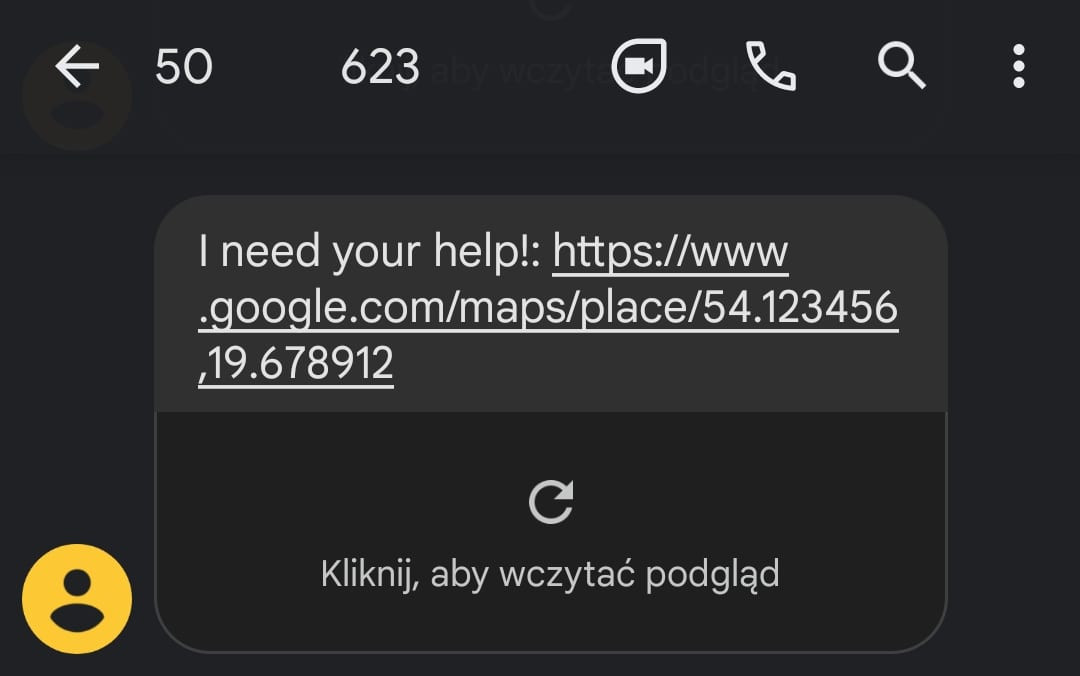
\includegraphics[width=6cm]{Graphics/sms.jpg}
    \caption{Odebrana wiadomość SMS z lokalizacją}
    \label{img:sms}
    \end{subfigure}%
    \vspace{1cm}
    \begin{subfigure}[b]{6cm}
    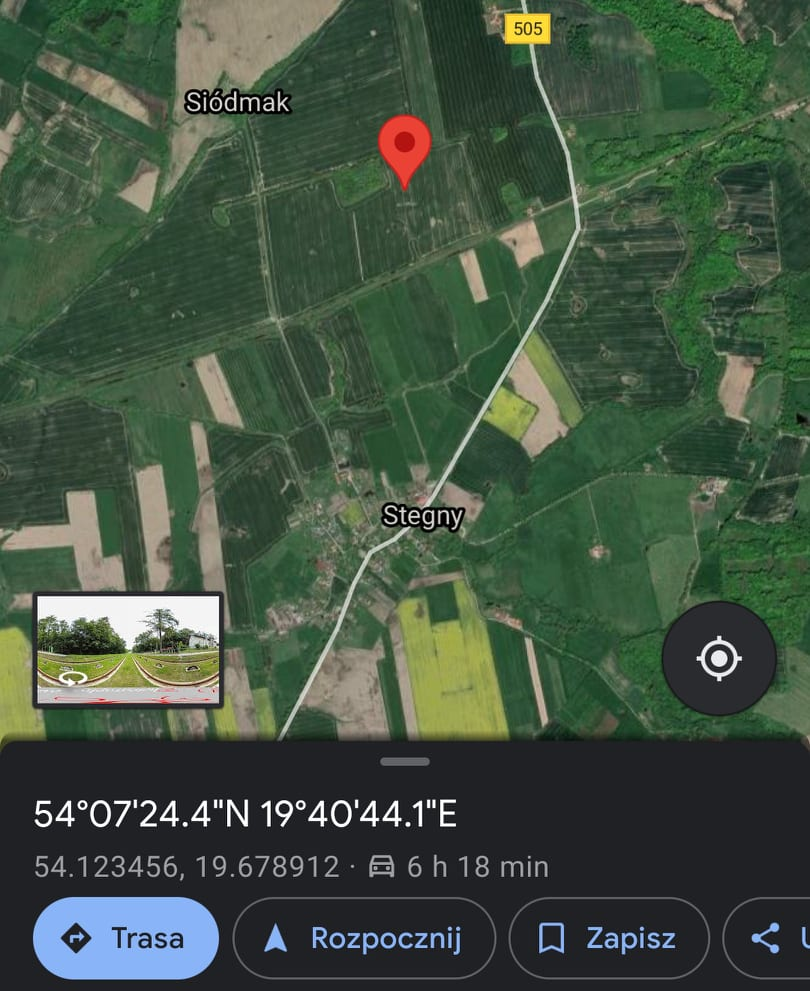
\includegraphics[width=6cm]{Graphics/maps.jpg}
    \caption{Lokalizacja na mapie Google}
    \label{img:maps}
    \end{subfigure}
    \caption{Wysyłane powiadomienie z lokalizacją}
    \label{img:notification}
\end{figure}
\chapter{Testy urządzenia}
\section{Analiza poboru prądu układu}
Zarówno w trakcie tworzenia pracy jak i jej planowania, zakładano minimalizację zużycia energii przez układ. Dzięki zastosowaniu odpowiednich komponentów, założenie to, zostało spełnione w bardzo dobrym stopniu. W trybie analizy, gdzie urządzenie spędzało znakomitą większość czasu, wartość pobieranego prądu spadała do nawet 200$\mu$A. Dzięki temu, stosując małe ogniwo Li-Pol o pojemności 600mAh, urządzenie mogło czuwać przez nawet 3000 godzin, co daje 125 pełne doby. Najwięcej prądu, pobierało pierwsze wyzwoleie alarmu. Średni pobór prądu sięgał tutaj nawet 50mA, w zależności od czasu potrzebnego na określenie lokalizacji. Kolejne transmisje nie były już tak energochłonne, ponieważ uruchamiany był tylko modem LTE.
\newline
Rysunek \ref{img:current_summary} przedstawia kompletną analizę poboru prądu przez układ. Obszar pierwszy, to obszar inicjalizacji urządzenia. To tutaj ustawiany jest każdy z komponentów i dokonywana jest pierwsza rejestracja do sieci. Należy zauważyć, że w tym miejsciu nie był uruchamiany GPS, co przyspieszyło inicjalizację układu. Strefa ta, jest tzw. selftestem, gwarantującym, że urządzenie będzie działać poprawnie w przypadku wypadku. W strefie drugiej, wszystkie podzespoły, znajdowały się w trybie głębokiego uśpienia. Wbudowane w akcelerometr maszyny stanów, cały czas monitorowały dane w trybie niskiego poboru energii. Na granicy obszarów 2 i 3, nastąpiło przerwanie. Uruchomiło ono procedurę alarmu, wyzwalając buzzer oraz uruchamiając GPS. Obszar 3 stanowiła próba określenia swojego położenia, a następnie przygotowanie i wysłanie wiadomości, poprzedzone rejestracją do sieci komórkowej. W obszarze czwartym, modem przeszedł w tryb uśpienia, a uruchomiony został licznik, który po minucie wyzwoliłby kolejne wysłanie wiadomości. Na granicy stref 4 i 5, nastąpiło przytrzymanie przycisku, które zakończyło alarm i wyłącza buzzer. Układ ponownie przeszedł w tryb analizy danych.
	

\begin{figure}[h]
    \centering
    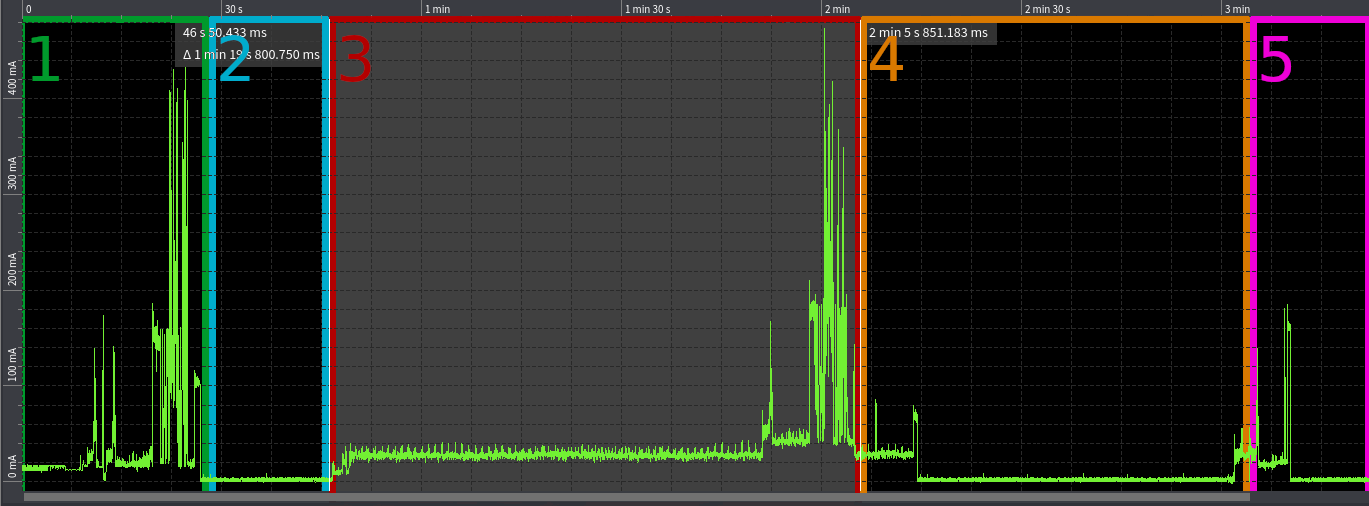
\includegraphics[width=14cm]{Graphics/connection_with_fix_divided.png}
    \caption{Analiza poboru prądu przy użyciu urządzenia otii}
    \label{img:current_summary}
\end{figure}

\section{Testy algorytmów}
Przyłożyć maszyny stanów do przebiegów i pokazać, że to się pokrywa
\chapter{Możliwości rozwoju urządzenia}
\chapter{Podsumowanie}
W pracy, podniesiono problem bezpieczeństwa samotnych rowerzystów, podczas wyjazdów górskich. Zdecydowano się zbudować urządzenie, mające poprawić poziom bezpieczeństwa na rowerze. W rozdziale pierwszym, określone zostały podstawowe wymagania, dotyczące układu. Podjęto też decyzję, o wykorzystaniu mikrokontrolera, akcelerometru, modułu GPS oraz modemu LTE. Dla każdego z podzespołów, dokonano analizy dostępnych rozwiązań, a następnie na jej podstawie, wybrano najlepszy z nich. Nie pominięto również przedstawienia podobnych rozwiązań, obecnych na rynku. Rodział drugi stanowi dokumentację z procesu tworzenia urządzenia. Stworzono prostą platformę do zbierania danych, wykorzystując dostępne układy oraz druk 3D. Korzystając ze stworzonego urządzenia, przeprowadzono eksperymenty, celem zebrania surowych danych. Dane te, przetworzono i poddano szczegółowej analizie. Wyniki, przekształcono w algorytmy, służące wykrywaniu wypadku rowerowego. Następnie, opisano logikę tworzonej aplikacji. Na potrzeby urządzenia, przetestowano dwa różne podejścia do analizy danych, wybierając bardziej energooszczędne maszyny stanów programowane w akcelerometrze. Opisano rówież procedurę pobierania przez urządzenie lokalizacji, kluczową dla poprawnego działania rozwiązania. Opisując implementację powiadamiania o zdarzeniu przy użyciu LTE, opisano dwie różne metody wysłania powiadomienia: zapytanie http oraz powiadomienie SMS. Ze względu na stabilność, zaimplementowano metodę drugą. Ponieważ wymagała ona wprowadzenia do kodu numeru telefonu, dodano stos Bluetooth, pozwalający na łatwe jego wpisanie do pamięci mikrokontrolera. W rodziale trzecim, przeprowadzone zostały testy wykonanego urządzenia. Przeanalizowano pobierany przez nie prąd oraz przedstawiono kolejne etapy działania na wykresie zależności prądu od czasu. Porównano również zaproponowane algorytmy do zebranych przebiegów, prezentując ich działanie. Rozdział czwarty stanowi opis możliwych kierunków rozwoju urządzenia oraz możliwości jego rozbudowy.



% itd.
% \appendix
% \include{dodatekA}
% \include{dodatekB}
% itd.

\printbibliography

\end{document}